\documentclass{UoYCSproject}
\usepackage{adjustbox}
\usepackage{graphicx}
\usepackage[nottoc,numbib]{tocbibind}
\usepackage{subcaption}
\usepackage[euler]{textgreek}
\usepackage{listings}
\usepackage{wrapfig}

\usepackage[utf8]{inputenc}
\usepackage[acronym]{glossaries}

\addbibresource{Report.bib}
\title{Parallel Programming Tools for Exploring Immune System Development}
\author{Oliver William Binns}
\MEng
\date{\today}
\supervisor{Dr. Fiona Polack, Dr. Kieran Alden}
\wordcount{10559}


%Approx 500 Words
\abstract{
More powerful computers are paving the way for sophisticated simulations of complex biological systems which are inaccessible to live \gls{in-vitro} study.
\acrlong{abm} has been previously used to implement this type of simulation \cite{kieran_thesis, kieran_methodology, flame_keratinocyte, stepney_abm}, showing how the behaviour of a number of individual agents can contribute to the system as a whole.

The desire to create larger and more elaborate simulations, while still ensuring results can be obtained in a reasonable amount of time, makes it necessary to use parallel and distributed systems.
Creating programs and simulations that make efficient use of this parallelism can be technically challenging.
In particular it requires implementing an optimal distribution of tasks over the system and ensuring the integrity of any memory that is shared across multiple threads.
Some significant problems, including a computer science skills shortage, are slowing down the rate of progress in this area.

This project investigates the challenges and advantages of using a parallel agent-based modelling platform, \gls{FLAME GPU}, by re-implementing an existing sequential simulation of the development of a small part of the immune-system, developed using \gls{MASON}.
During the building of the simulation, I have discovered that it is not trivial to compare between the old and new implementations, due to differences in the frameworks used.
For this reason, the final comparison will be done directly to the domain model itself.

Finally, in order to improve the mapping from the biological domain model to \gls{FLAME GPU} simulation code, I propose a \acrlong{mde} approach to development.
This approach reduces the parallel computing skill required to develop \gls{FLAME GPU} implementations and improves traceability from the biological domain to the implementation.
%add a little bit about the experiments you have carried out (very brief)
%and a general account of the significant findings (including any drawbacks)
}

\acknowledgements{
I would like to thank my supervisors, Fiona Polack and Kieran Alden, for their support and guidance throughout this project.
\\

I also express my thanks to Richard Paige for his pastoral support throughout this academic year, as well as his help in obtaining access to a suitable \acrshort{gpu} machine.
\\

Finally, I would also like to thank the \gls{FLAME GPU} development team at the University of Sheffield for their help in utilising the latest and pre-released features of this framework.
}

\makeglossaries
\newacronym{abm}{ABM}{Agent-Based Modelling}
\newacronym{cosmos}{CoSMoS}{Complex Systems Modelling and Simulation Infrastructure}
\newacronym{cpu}{CPU}{Central Processing Unit}
\newacronym{cuda}{CUDA}{Compute Unified Device Architecture}
\newacronym{evl}{EVL}{Epsilon Validation Language}
\newacronym{egl}{EGL}{Epsilon Generation Language}
\newacronym{flame}{FLAME}{Flexible Large Scale Agent Modelling Environment}
\newacronym{flamegpu}{FLAME GPU}{\acrshort{flame} for the \acrshort{gpu}}
\newacronym{gpu}{GPU}{Graphics Processing Unit}
\newacronym{gpgpu}{GPGPU}{General Purpose \acrshort{gpu} programming}
\newacronym{lto}{LTo}{Lymphoid Tissue organiser cell}
\newacronym{ltin}{LTin}{Lymphoid Tissue initiator cell}
\newacronym{lti}{LTi}{Lymphoid Tissue inducer cell}
\newacronym{mason}{MASON}{Multi-Agent Simulator Of Neighborhoods}
\newacronym{mde}{MDE}{Model-Driven Engineering}
\newacronym{mimd}{MIMD}{Multiple Instruction, Multiple Data}
\newacronym{mpi}{MPI}{Message Passing Interface}
\newacronym{simd}{SIMD}{Single Instruction, Multiple Data}
\newacronym{ycil}{YCIL}{York Computational Immunology Lab}

%behavioural model
%complex meaning
\newglossaryentry{domain}
{
    name=Domain Model,
    description={A conceptual model which details the behaviour and data of a real-world system}
}
\newglossaryentry{platform}
{
    name=Platform Model,
    description={A formal specification stating how ambiguous aspects of a domain model should be implemented in simulation code}
}
\newglossaryentry{FLAME GPU}
{
    name=\glslink{flamegpu}{FLAME GPU},
    description={An extension of the \acrshort{flame} framework which uses \acrshort{gpu}s for parallelism}
}
\newglossaryentry{Host}
{
    name=Host,
    description={In \acrshort{gpgpu} programming, the computer containing the \acrshort{gpu} is referred to as the host}
}
\newglossaryentry{Device}
{
    name=Device,
    description={In \acrshort{gpgpu} programming, the \acrshort{gpu} hardware being used, is referred to as the device}
}
\newglossaryentry{PP}
{
    name=Peyer's Patch,
    description={Clusters of cells that form in the small intestine}
}
\newglossaryentry{LTi}
{
    name=\glslink{lti}{LTi},
    description={A moving cell that can bind to any static cell. Believed to be responsible for initiating \gls{PP} development}
}
\newglossaryentry{LTin}
{
    name=\glslink{ltin}{LTin},
    description={A moving cell that can bind to any static cell. Responds to chemokine expression}
}
\newglossaryentry{LTo}
{
    name=\glslink{lto}{LTo},
    description={A static cell. Divides on stable bind with an \gls{LTin} and \gls{LTi} cell}
}
\newglossaryentry{Chemokine}
{
    name=LTo,
    description={Scientific tests conducted using computer simulation}
}
\newglossaryentry{MASON}
{
    name=\glslink{mason}{MASON},
    description={\href{https://cs.gmu.edu/~eclab/projects/mason/}{A Java framework} for producing simulations using \acrshort{abm}}
}
\newglossaryentry{in-silico}
{
    name=in-silico,
    description={Scientific tests conducted using computer simulation}
}
\newglossaryentry{in-vitro}
{
    name=in-vitro,
    description={Scientific tests conducted using real biological systems under laboratory conditions}
}


\begin{document}
\pagenumbering{roman}
\maketitle
\listoffigures
\printglossary[type=\acronymtype]
\printglossary


%Approx 1000 words
\chapter{Introduction}
\pagenumbering{arabic}
%TELL THEM WHAT YOU WILL TELL THEM
%LIT REVIEW: TELL THEM
%RESULTS/EVAL: TELL THEM WHAT YOU TOLD THEM!
\gls{abm} has been successfully used to simulate biological systems and develop new scientific knowledge \cite{kieran_thesis, flame_keratinocyte}.
While traditional mathematical-based models are generally much more efficient to compute and produce good results when exploring how biological factors effect populations as a whole, \gls{abm} is particularly useful when considering how individuals and their interactions produce emergent system behaviour.
Mathematical-based models are limited in this aspect as they assume that each individual within the population is identical.
\gls{abm} explicitly represents each individual, meaning these can have state and attributes and are independent and fully autonomous.
Often this behaviour is stochastic meaning that each execution of the simulation produces different outputs even with the same initialisation.
This stochastic behaviour means that a large number of executions are required to ensure statistical significance.
This means that as agent-based simulations become more complex, they require significantly more compute resources to produce results within a realistic period of time.

Here, and throughout this report, the term complexity does not necessarily refer to simulations that contains several components that are difficult to engineer.
Rather, we discuss simulations that are made up of lots of simple components that interact with each other and the environment in such a way that the system behaviour is so elaborate that it can only be predicted by running the simulation.

As these simulations often contain non-deterministic behaviour, numerous runs are required to ensure that results are statistically significant.
Consequently, it is important to ensure that the simulations make efficient use of the available compute resources, in order to gather these results in a reasonable amount of time.
The inability to obtain simulation results in a reasonable time is one of the most significant constraints upon the current use of agent-based simulations within biological research.

Another constraint affecting the adoption of \gls{abm} simulations is the ease with which they can be created.
At present, domain experts with knowledge of a particular biological system produce domain models of the system.
With the aid of software developers, these domain models are then converted into platform models.
The domain experts verify that the platform models are reasonable abstraction of the system, and they are implemented in code by the software developers.
This is the \gls{cosmos} process (Fig. \ref{fig:cosmos_process}).
\label{cosmos_intro}

\begin{figure}[htp]
\centering
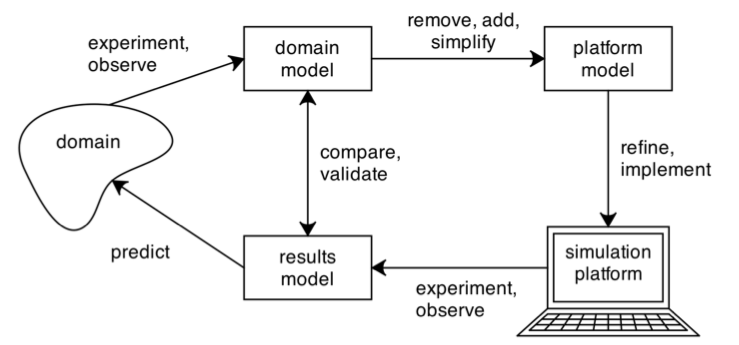
\includegraphics[width=0.75\textwidth]{Appendix/CoSMoS_Process}
\caption{\gls{cosmos} Process (Taken from \cite{mark_read_thesis})}
\label{fig:cosmos_process}
\end{figure}

A shortage of software developers who are proficient at creating efficient, parallel simulations is the current bottleneck in the adoption of the \gls{abm} simulations of processes.
If this development process can be automated by creating general solutions for common biological processes, such as cell division, it will allow simulations to be created by domain experts.
%this report discusses limitations, that are preventing this process being used to its full potential
%and explores potential solutions to this..!

%an introduction to what is to follow
%the abstract can be very specific
%Here: a bit more general (i.e. MDE and simulation concerns in general)

\section{Motivation}
%What can be gained from better modelling.. particularly biology..?
%Presentation- see justification slides!
The motivation behind this project stems from the new knowledge that could be gained from the ability to easily create efficient, parallel biological simulations.
As many biological systems cannot be fully studied \gls{in-vitro}, simulations can provide a valid alternative.
Indeed previous work has been used to produce novel biological hypotheses which have been shown to be statistically similar to those observed in the laboratory \cite[p.174]{kieran_thesis}.

%do we need citations/examples here if we are going to discuss this in more detail later on?
%is it ok to reference a later chapter?
However, these previous simulations of biological systems have had to make significant trade-offs in their implementation.
For example, 3D environments have had to be mapped into 2-dimensional simulations, cell migration into the system has been modelled as random rather than systematic \cite{kieran_thesis}, and environmental growth has been ignored \cite{phil_diss}.
%number of cell types have been reduced
The impact that these compromises have on the validity of the platform model as a representation of the domain is currently unknown.
A core motivation of this project is that, by addressing the difficulties of creating efficient, parallel, agent-based simulations, we can support simulations with fewer trade-offs in their realisation.
%can also increase the scale of the simulation

%outside of biological exploration, new understanding can..?
There are several compelling reasons for the interest in simulation of immune-related biology.
Firstly, extensive \gls{in-silico} testing could be performed much more quickly than the current \gls{in-vitro} testing, reducing the time it takes to research new drugs and cures.
Drugs and cures would be available for patients earlier, saving many lives.
Additionally, the significant financial burden of drug development, which is estimated to be around \$2.9bn \cite{drug_cost}, could be reduced, freeing up heavily contested funds for additional research. Finally, the use of animal testing could be reduced and, in the long term, eliminated completely.

\section{Project Aims}
\label{aims}
In summary, the aims of this project are to
\begin{enumerate}
    \item Establish a firm grounding for the future development of new tools to allow fast, parallel simulations of biological systems to be easily created by non-technical users.
    \begin{enumerate}
        \item Explore the findings of the new implementation and discuss how these can be generalised between different simulations.
        \item Discuss techniques for allowing non-technical users to easily create formal models that can be transformed into new simulation implementations.
    \end{enumerate}
    \item Develop a \textbf{parallel} implementation of an existing \textbf{sequential} simulation of \gls{PP} development and explore any speed increases that can be produced by using \gls{gpgpu}.
    \item Review the use of simulations, with a particular focus on computational biology. This review explores the advantages that in-silico testing provides over \gls{in-vitro} experimentation and the problems that must be overcome for the mass adoption of biological simulations.
    
\end{enumerate}

\section{Statement of Ethics}
This project was conducted in accordance with the University of York's code of practice on ethics.
This project does not involve human participants, so guidelines on informed consent and confidentiality will be met. No confidential medical data or personal information has been used during the course of the project development. This project has involved no direct animal participation.
%[Where did the data come from?!], how was the original model created, should this be mentioned?

The ability to reduce, and ultimately replace, experimentation on animals is a positive ethical advantage of work on efficient immune-related simulation.

The simulation of the biological model is for the purpose of developing understanding of applying \gls{gpgpu} methods to an agent based model of a biological system. It will not be used its current form to publish novel biological findings and does not fully simulate a biological process.
%Software used and licences? FlameGPU is freely available / open source
%Cuda is proprietary but freely available..
%Hardware.. is this relevant?

\section{Report Structure}
This report details the work done throughout the project and 

\begin{itemize}
    \item Chapter \ref{lit_review} gives an overview of simulations and the benefits and limitations of their use particularly with regard to computational biology.
    \item Chapter \ref{tools} states the tools used to facilitate the implementation of the new \gls{FLAME GPU} simulation and presents details of model that was simulated.
    \item Chapter \ref{methods} details the development of an improved, inherently parallel, implementation of PPSim (\textit{PPSim v2}) and the \gls{mde} tools that were developed to aid this work.
    \item Chapter \ref{results} evaluates the progress that this project has made towards making \textbf{fast}, parallel simulations more \textbf{accessible}.
\end{itemize}

%Approx 3000 words for literature review
\chapter{Literature Review}
\label{lit_review}
% Aims are to:
%
% Place original work into the context of existing Literature
% Interpret major issues surrounding the topic
% Describe the relationship of each work to the others under consideration 
% Identify new ways to interpret, and shed light on any gaps in previous research
% Resolve conflicts among seemingly contradictory studies
% Determine which literature makes a significant contribution to your understanding of the topic
% Point your way to further research on your topic

\section{Simulation Background}
\label{simulation}
%Background, what are simulations used for generally
Simulations are model-based imitations of a system which feature its key characteristics and behaviours.
The system being modelled is referred to as the domain, while this simulation is known as the platform.
Computer simulations are used in a wide range of disciplines on applications such as video games, medicine \cite{abm_case_studies_ycil, healthcare_population}, product development \cite{sim_manufacturing} and even nuclear weapons \cite{nuclear_simulation, gizmodo_nuclear}.

The models of systems used in simulations may have a varying amounts of abstraction.
Simulations used for teaching will likely have models which remove significant amounts of complexity from the system.
Using abstraction to remove some of the complexity present in the domain can also help to reduce the time it takes to run the simulation, a key focus of this project.
Simulations used for video games tend to be as realistic as possible as realism has been shown to produce a higher level of immersion \cite{realism_immersion}, a highly desirable attribute of games.
%mention speculation that we live in a simulation? - simulation hypothesis, The Matrix, Elon Musk

%ABM...
In particular this project will focus on simulations created using \acrfull{abm}.
\gls{abm} is a technique that explores the autonomous behaviour and interaction between a number of individuals, known as agents.
The aim of this is to show how the individuals' behaviours interact to produce the system as a whole.
This is in contrast to more traditional mathematical top-down models which consist of a set of equations which establish relationships between a set of variables.

%Simulations have been a major focus of the \href{https://www.york.ac.uk/computational-immunology/}{\gls{ycil}}\cite{abm_case_studies_ycil}, a group combined of domain experts (immunologists) as well as modellers (engineers, mathematicians) and software developers (computer scientists).
%so what?

This chapter begins by outlining the benefits and current limitations of using simulations \textit{generally}.
It then discusses some potential solutions to some of these limitations before applying this to some of the existing simulations that have been developed using \gls{abm}.

\subsection{Benefits}
\subsubsection{Feasibility}
Exploring computer simulations is can be far more feasible than exploring a real world environment.
Video games are simulations which may allow players to experience scenarios that they may not otherwise get the opportunity to encounter.
For example, car racing games are significantly cheaper and safer than real life racing.

Real-world scientific testing may not be feasible for a number of reasons.
Simulating the aerodynamics of new car designs virtually is far quicker and cheaper than creating multiple different prototypes for physical tests.
Morality may be a factor, a good example of this is animal testing for cosmetic products or medicine.
With nuclear weapons, legality too is a key issue, as some weapon testing is banned under a number of global treaties \cite{partial_nuclear_test_ban_treaty, threshold_test_ban_treaty}.
Finally, some real-world tests may be too dangerous to perform, such as in the case of invasive medical examinations.
%SO WHAT? %POINT, EVIDENCE, EXPLANATION:
In all of these examples, computer simulation is routinely used to reduce or replace real-world testing.
%can scale be a factor? simulations can quickly model across numerous independent variables - see environmental control

\subsubsection{Reducing Complexity}
Reducing complexity through abstraction allows better understanding of the system to be gained as the complexity may initially be overwhelming.
%Removing complexity can help with understanding by removing aspects of the system that are not absolutely essential to the functionality being demonstrated.
Abstractions need to be made to an appropriate layer, models should represent the layer being investigated, but remove any unnecessary further detail.
For example, attempting to model simulations exploring cell development down to the atomic or quantum level or up to an entire organism would be completely unnecessary.
Attempting to do so with current technology would also be completely untenable.
This is an important balancing act as, if too much detail is abstracted away, simulations will likely fail to produce the expected emergent behaviour \cite{stepney_abm}.
%todo: talk about abstracting to appropriate layers..
%   clearly we only want to simulate the individuals at the level we are interested in
%   i.e. we obviously don't want to simulate our models down to the atomic/quantum level, etc.

\subsubsection{Environmental Control}
Computer simulations allow for the environment to be more easily controlled.
While the initial setup of a realistic environment may be difficult, once this has been achieved the simulations can be run in a known, constant environmental context.
The ability to adjust external factors and independent variables that may affect the system on demand can be particularly useful.
In \gls{in-vitro} testing, the environment often changes in unknown, unpredictable and, most importantly, \textit{unrepeatable} ways.
\Gls{in-silico} experimentation can ensure the test environment remains unaffected by any external factors.
This ability can be used for illustrating how different variables affect system processes.

%Time can be manipulated to visualise system processes at more reasonable time scales.
%A chemical process that takes a fraction of a second can be slowed down to ensure that it can be seen. 
%speed up, reverse the simulation
%easier to measure?

Furthermore, simulations allow for additional tests to be easily added at a later date.
For example, if measurements are not made for a particular variable, it can be easily added to the implementation and the simulation can be easily re-run.
This is not the case with in-vivo experimentation, which would require the laboratory to be fully set-up again, with new test-subjects for repeat experiments.

%clearly simulations may be more feasible but
%WHY are they a good alternative to real world testing?!
%accurate/realistic results produced
    %when is this the case? always? when sufficient knowledge is known?
    %relate this to laws of Physics, theoretical biology?

\subsubsection{Visualisation}
\label{visualisation}
One of the biggest benefits of simulation is the ability to graphically visualise a system or its constituent parts.
Using simulation for visualisation has number of benefits over attempting to demonstrate real world systems.
Several of these benefits translate from the previous two sections- they can be more feasible to explore than a real world environment and featuring a reduced complexity can allow the key concepts to be understood without overwhelming the user.

Simulation can be particularly useful for visualising concepts for education. 
Particularly immersive educational visualisations can also be produced using virtual and augmented reality.
The Virtuali-Tee is an educational tool that uses simulation and augmented reality to provide a view at the body's internal organs \cite{curiscope}.
Little Journey aims to reduce kids' anxiety about surgery by providing a realistic tour of their hospital ward given by animated cartoon characters \cite{little_journey}.
%use a paper to show that these are actually "immersive"

%TODO: visualisations using the CPU are VERY computationally expensive

%visualisations from the given models may not be fully accurate / may be misleading:
%   often only time-series or single-time data is available to calibrate and test the simulation..!

\subsection{Limitations and Constraints}
%ARE THERE ANY CONS?
%SHOULD simulations be used by everyone?
%Why are they not?
While simulations seem very useful across a wide number of fields, there are some significant limitations as to where and how they can be used.

\subsubsection{Insufficient Domain Knowledge}
\label{domain_knowledge}
A simulation is based on a model of a system.
A model is an abstraction from reality representing only the necessary key characteristics and behaviours of the system.
In order for the model to the be faithful to its original domain it must be able to produce demonstrably similar behaviour from similar system components.

A lack of knowledge regarding the domain of the simulation is one of the most significant constraints regarding its implementation.
If this is the case, the model produced may be incorrect or abstractions may remove necessary detail required for the system to function as expected.
With biological simulations in particular, it is often hard to make assumptions about how particular processes occur \cite{stepney_abm}.
Unfaithful models can also be a result of \textit{incorrect} knowledge of the domain.
For complex systems, having too many abstractions from the original domain may also invalidate the model and produce incorrect results \cite[p.8]{cosmos}, \cite{stepney_abm}.

While knowledge of a system needs to be sufficient to produce reasonable assumptions, it need not be perfect.
This is particularly the case with the type of simulation discussed later in this report (Section \ref{platform}).
In this case, the \gls{platform} makes assumptions about the domain, in order to allow a concrete implementation.

\subsubsection{Compute Power}
Complex models with too few abstractions from their domain may require significant computing power to simulate.
Additional abstractions may not be possible as they may invalidate the model \cite{stepney_abm}.
In \gls{abm} simulations, even simple models may be computationally difficult if a large number of agents or interaction are required to emulate reality.
In these cases, cutting edge hardware may be needed for the simulation to be run in an acceptable time.
Powerful hardware is expensive to access, so this may be a significant constraint on the ability to simulate.
%Agent-Based Modelling, which will be introduced in detail in Section \ref{abm}, models the system as a number of autonomous individuals. This technique requires significantly more compute power than the traditional top-down simulations.

%Talk about the need to speed up
%evidence behind this--!
    %machine learning paper- drive to better capture biological complexity
    %video games, better graphics and more detail
    %other examples?

%only get data on variables that have been modelled, whole system is likely not modelled, see TWA Flight 800...:
%The NTSB deemed a physical simulation appropriate as they were not convinced an available computer model would confirm the true cause of the accident.


\subsubsection{Skills Shortage}
\label{skills_shortage}
The previous section discussed reliance that complex simulations have on the latest advanced hardware capabilities.
However, advanced hardware alone will not necessarily allow a simulation to compute in a reasonable amount of time. 
%mention the concurrency- free lunch is over article findings
With modern architectures which are becoming increasingly parallel, the simulation code must be tailored to take advantage of the computing power available.
Efficient parallel programs that do this rely on the availability of experienced programmers.
Many recent studies have highlighted the existence of significant computer science skills shortages, across the world \cite{digital_skills_uk, microsoft_blog}.
These skills shortages may be significantly limiting the possibility for cross-disciplinary work to utilise fast, advanced simulations.

%Computer science degrees, and related courses and apprenticeships, are proving less popular in recent years
%These are worrying trends considering the demand for digital skills by employers
    % - DIGITAL SKILLS for the UK ECONOMY, A report by ECORYS UK, JANUARY 2016

%Put simply, our nation faces an increasing shortage of individuals with the skills necessary to create and deploy the next generation of information technology.
%Despite the growing importance of computer science, it is only taught in a small percentage of U.S. schools. 
    %Microsoft Corporate Blogs, https://blogs.microsoft.com/on-the-issues/2012/12/12/investing-in-american-innovation-and-the-next-generation/

Many initiatives are being rolled out to address this issue.
Computing was added to the National Curriculum in 2013 \cite{national_curriculum, teacher_training} and numerous technology companies are also creating their own campaigns \cite{apple_education, microsoft_education}.
It is likely that these will take a number of years to yield results, but should eventually mean that even domain-experts have a basic grasp of code.

\subsubsection{Bugs}
As with any form of computer program, mistakes can be made causing bugs to be present in the simulation code.
Bugs may cause the simulation to be incorrect meaning any hypotheses and results are based on incorrect data.
This is linked to, but not the same as, having insufficient domain knowledge.
Both of these limitations will cause the simulations to fail silently, produce incorrect results with no immediately obvious failure.
%Failing silently is interesting: no unexpected behaviour.. this should be discussed in more detail
Third-party tools, such as \gls{abm} libraries, that may be relied on are not bug free.
Indeed, no software can be shown to be bug-free as testing only shows the presence, not the absense of bugs \cite[p.16]{dijkstra}.
As part of this project, a major bug which has been present in the code for the \gls{MASON} \gls{abm} framework since February 2013 was discovered and fixed \cite{mason_pull_request}.


However, while these problems are specific to simulation, they are not dissimilar from the issues that can occur from poorly designed real-world testing.
%GIVE MORE DETAIL HERE: how can poorly designed in-vitro testing affect results in similar ways?
In real-world testing, poorly designed experimentation is often the only available approach.
When gathering time-series data regarding immune-system development, the process of obtaining the data is destructive.
At each point in the series, a mouse is dissected and the data gathered.
The different animals used throughout the time-series have the potential to introduce a large element of unreliability in the results.

Furthermore, even when \gls{in-vitro} experiments are well designed, statistical analysis can lead to misleading results.
Comparisons using a t-test are common but almost always invalid as they incorrectly assume that the results will fit a particular mathematical distribution.
In reality it is almost impossible to demonstrate that experimental data fits the criteria for a given distribution \footnote{Personal communication, \href{http://www.scm.keele.ac.uk/staff/f_polack/}{F. Polack}}.
As such, errors in the simulation tests is no reason to dismiss simulation as an alternative to real world testing in general.

%Here we are talking about refining from an initial model, which we have shown to be correct:
%This is the same concept as MDE - discussed later!
If the simulation needs to be safety-critical, developing it using formal methods and refinement may be a good way to ensure that no bugs are introduced in the code.
This refinement is a similar in concept to the \gls{mde} techniques for model refinement that will be presented in Section \ref{methods} of this report.
%CSP -> OccamPi/MASON -> Kieran is currently looking into this
%Similar to the work described later in this report: model-driven engineering!
%ensures that artefacts are inline with each other

\section{Existing Simulations}
%Previous implementations of simulations and their problems:
%In order to achieve mass-market userbase, they must be:
%EASIER TO MAKE - less technical users can work on them
%FASTER TO RUN. - more feasible, to use in experiments, more complex sims can be made

\subsection{Biological Simulations}
Computational Biology is a relatively new field of study that has been growing significantly over the last decade[CITATION NEEDED].
Within Biology, simulation is often required as an alternative to invasive medical testing/animal testing.%NC3Rs
Simulation has even been proposed as a method for exploring a potential set of first principles and mathematics that are specific to biology which could even constitute a new subject- theoretical biology \cite{rise_article}.

\subsection{\acrlong{abm}}
\label{abm}
As previously mentioned, \gls{abm} models the autonomous behaviour of individual agents and the interaction between them.
%Write comparison of AGENTS vs OBJECTS (OOP)
Agents are often confused with objects, a commonly-used programming concept.
However, it is important to emphasize the differences between them.

In particular, while both agents and objects recognise the importance of interactions, objects are totally obedient to their method calls whereas agents have autonomy \cite{abm_v_objects}.
This means that agents can interact and react to communications according to their own agenda.
Moreover, agents and objects persist differently.
Agents, like biological cells, may evolve into a different state to take on different behaviour.
In contract, in order to follow the single responsibility principle \cite[p.95]{srp}, when object behaviour needs to change, the object will generally be deleted and replaced with an object of a new class.

%WHY IS AGENT BASED MODELLING THE MOST RELEVANT FOR THIS PROJECT
While, \acrlong{abm} is more computationally expensive than top-down mathematical modelling, it is also more natural to model and intuitive to parallelise \cite{flame_simulation}.
Communication between individual agents can be difficult to implement in parallel but parallel communication is by no means limited to \gls{abm}.
The challenges of parallelising agents is a the key challenge of this and other related projects \cite{andy_proj, jeff_proj}.

\subsubsection{Custom Code}
This report builds on an existing custom code example of \gls{abm} simulation which utilised \gls{gpu} parallelism \cite{phil_diss}.
%quick background of this
This simulation was built on a tried and tested domain model of \gls{PP} development \cite{kieran_thesis}.
%findings
The simulation was successful in demonstrating the development of \gls{PP}es described in its domain model.

However this is not always the case.
A custom code \gls{abm} simulation was used to investigate the processes of auxin transport in plants \cite{stepney_abm}.
%background:
The simulation focused on how the transport canals in the stems of plants develop.
%findings:
Unfortunately this simulation did not produce the auxin transportation canals that would be expected from the biological model.

While it is clearly possible for agent-based simulations to be created from scratch there are several distinct disadvantages to doing so.
Firstly, using existing frameworks avoid programmers having to reinvent the wheel, massively reducing the amount of code that they need to produce.
As well as saving a significant amount of time, commonly used frameworks are often well tested making software bugs less likely.
%parallelism must be ensured.
%not well tested?
Furthermore, unlike simulations that are created using \gls{abm} libraries, they do not inherit any support for new tools and hardware that come from updates to the library.
In contrast, custom code simulations must each be updated separately with any enhancements required for new hardware capabilities.

\subsubsection{Proprietary Solutions}
Some proprietary solutions are available to aid the creation of efficient \gls{abm} simulations.
One example of this, with a reasonable level of industry support, is Biocellion \cite{biocellion_paper}.
While it is freely-available for non-profit use, it does not help with our aim of creating a simulation platform that is simple-to-use.
While it makes the task of creating efficient parallel simulations which are portable far simpler, it requires a level of proficiency with the Linux OS, C++ programming and familiarity with mathematical modelling concepts.
In particular, we cannot expect domain experts to be proficient at C++ programming.
Software engineers will still be required in the simulation development process.
In the future productivity layers which allow simulations to be created by less technical users will be added to Biocellion, but these are not yet available \cite{biocellion_paper}.
Biocellion's closed source approach rules out the ability for us to build on this work, while a license agreement has hindered adoption \cite{physicell}.

%unfortunately, technical to understand- took several weeks to even install, how to cite conversation? CITE Jeff's report?

\subsubsection{\gls{MASON}}
%mason usage
\gls{MASON} is a multi-agent simulation library for Java.
%REMEMBER, this section is on EXISTING SIMULATIONS: discuss what MASON has been used for!
Many of the simulations developed by \gls{ycil} for exploring the immune system have used \gls{MASON} \cite{kieran_thesis, leishmaniasis, leukocyte, abm_case_studies_ycil}.
\gls{MASON} has been previously evaluated as the one of the fastest ABM libraries available \cite{abm_platforms_review}, however this evaluation took place over a decade ago and does not factor in any of the recent work into \acrshort{gpu} parallelism \cite{flame_simulation, biocellion_paper, physicell}.
Meanwhile, \gls{MASON} only supports \gls{cpu} parallelism, this will be discussed in more detail in Section \ref{cpu_v_gpu}.

\subsubsection{\gls{FLAME GPU}}
\label{flame_gpu}
The \gls{flame} project is an attempt to make \gls{gpu}-based \gls{abm} simulations more accessible.
This framework is covered here in more detail because it is a key tool used in this project.
\gls{flame} simulations consist of two artefacts, an `XML Model File' containing the structure of agents and their channels of communication and C source code file of `Scripted Behaviour' which defines the actual behaviour of agents.
\acrfull{flamegpu} is an extension of the original version of \acrshort{flame}, where the simulations that are created are compiled down to parallelised CUDA code.
%flame is built on top of CUDA, why?
This means the simulation can take full advantage of the power of modern NVIDIA \acrshort{gpu}s.

\begin{figure}[htp]
\centering
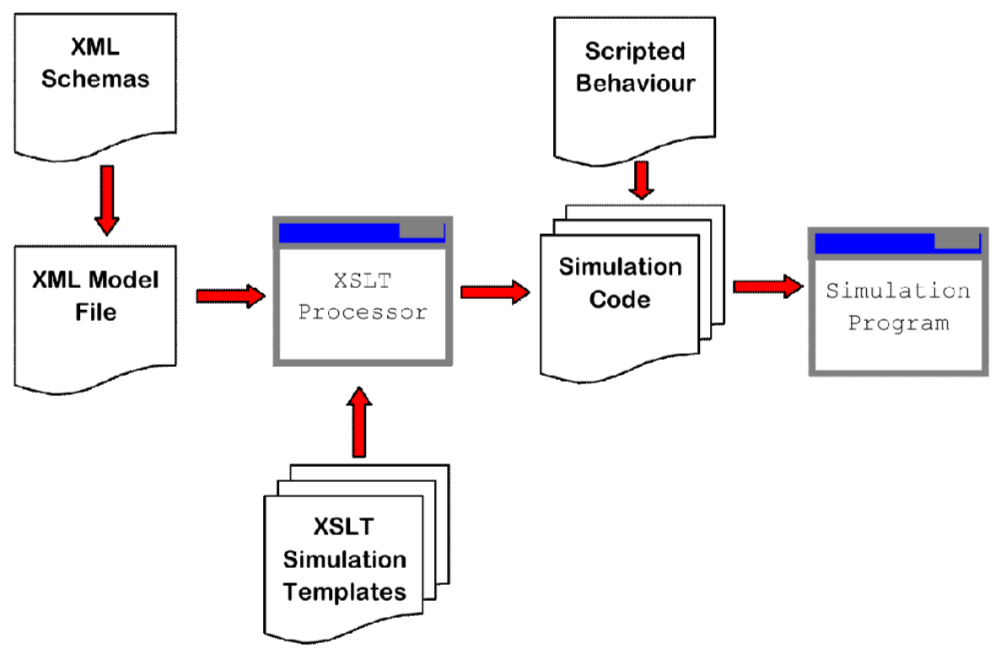
\includegraphics[width=0.6\textwidth]{Appendix/FLAME_Process}
\caption{\gls{FLAME GPU} Development Process (Taken from \cite{flame_simulation})}
\label{fig:flame_dev}
\end{figure}

\gls{flame}'s use of \gls{mde} could gives domain experts with limited programming knowledge the ability to understand and help design the simulation models, however a software engineer is still needed for the final implementation.

%partitioning is particularly effective if the vast majority of space is unpopulated
%Other specifications of FLAME GPU?

%REMEMBER, this section is on EXISTING SIMULATIONS: discuss what FLAME has been used for!
\gls{FLAME GPU} has previously been used for a number of large-scale simulations \cite{flame_pedestrian, flame_largescale}.
It has also been used in \gls{in-silico} biological experiments \cite{sperm_3d, maternal_interactions}, including an example at cellular level \cite{flame_keratinocyte}.

%Disadvantages
While relying on a framework such as \gls{FLAME GPU} can cause problems if support is stopped, this should be slightly less of a concern as \gls{FLAME GPU} is an open source project.
A more pressing concern with relying on any framework is that implementations are restricted by any of the framework's limitations.
For example, the current stable release of \gls{FLAME GPU} does not allow new agents to be created by the \gls{Host} between simulation steps.
%other limitations?

%Advantages
However, the \gls{FLAME GPU} framework does bring a number of advantages.
Firstly, it provides a \gls{mpi} which abstracts away from the underlying agent communication.
This \gls{mpi} supports spatial partitioning allowing messages to be passed only to nearby agents.
Communication between threads which is one of the most difficult tasks in parallel programming.
\gls{FLAME GPU} manages this communication in its entirety, meaning programmers can instead focus on ensuring the agent behaviour is correct.

%VISUALISATION COMES FREE!
\gls{FLAME GPU} also provides visualisations for simulations straight out of the box.
The benefits of visualisation are discussed in Section \ref{visualisation}.
Visualisations in \gls{FLAME GPU} run in real-time and can be useful for quickly verifying whether a simulation is behaving as expected.
%SCREENSHOT FIGURE HERE?

Many other advantages come directly from \gls{FLAME GPU}'s use of \gls{mde}.
\gls{FLAME GPU} is continuously updated to support new hardware advances, such as multicore \acrshort{gpu} architectures \cite{flame_simulation}.
\gls{FLAME GPU} simulations can always be certain of taking advantage of the latest hardware optimisations and portability features that the framework provides.
Existing simulation models that are implemented on top of \gls{FLAME GPU} may receive these performance improvements without any major code changes.
%In particular, it gives domain experts with limited programming knowledge the ability to understand and help design models.
%Additionally, the auto-generation of artefacts, such as simulation code templates, significantly lowers the boundary to entry to less advanced programmers.

Some notable benefits of \gls{mde} are not exploited in the current implementation of \gls{FLAME GPU}, these will be discussed later in this project (Section \ref{ppsim_v2}).
%TODO discuss these:
%migration?
%auto-generation
%auto-validation fixes?

\section{Improving Simulations}
\label{improvements}
%Section on what we need to support complex simulations
%link this to the previous chapter- discussion on current constraints on simulation:
Significant constraints on when simulations can be used were discussed in Section \ref{simulation}.
In order for simulations to become more widely adopted, some of these constraints must be overcome. 
In particular, this project focuses on two particular sections of which I believe will have the biggest immediate impact.
This section discusses the potential solutions to each of these problems.

\subsection{Ease of Creation}
\label{ease-of-creation}
A major constraint on the adoption of simulations is how difficult and time-consuming they are to create.
This constraint is exacerbated by a current shortage of experienced programmers.
Initial work to help overcome this skills shortage will likely come by providing tools that can automate work done undertaken by technical users as a means to increase their productivity.
Eventually, if this technical work can be fully automated, non-technical users will be able to easily create advanced simulations.
%person-centric healthcare, custom simulations may be needed

%difficult to create a framework that allows for easy modelling of BOTH state and interaction between agents[CITE NEEDED?, no but seriously]

%As computers are getting easier to use, users are beginning to expect this even from advanced tools

\subsubsection{\acrlong{mde}}
This project has already discussed abstractions with regards to modelling for simulations.
Abstractions are also particularly useful in software engineering.
As software gets more complex, additional abstraction is generally needed in order to extract the important details of the implementation \cite[p.24]{csapp}.

\gls{mde} is a software abstraction for creating and exploiting domain models, such as those that have been previously discussed with regards to simulations.
\gls{mde} has shown a promising increase in understanding between stakeholders and can produce productivity gains when models are reused across projects \cite{mde_industry_review}.

%EPSILON, benefits of MDE?
%Domain specific modelling, etc.

\paragraph{Epsilon} Epsilon is a set of tools and languages for supporting \gls{mde}.
Epsilon provides both the standardised modelling and metamodelling languages and model management technologies that are required for successful \gls{mde} projects \cite{eol}.
It provides tools for creating metamodels for new domain specific languages.
Epsilon facilitates model validation, model-to-model transformation and code generation to be performed on for models conforming to this metamodel. \cite{epsilon_book}

%Tools are a particularly important feature of mde.
%According to its website, Epsilon has a wide range of industry support.

\paragraph{Flexible Modelling}
Flexible Modelling tools could be a good method for allowing new simulations to be created more easily.
Using flexible modelling, non-technical users would be able to create sketches which can be automatically processed by tools into formal models and prototype metamodels \cite{Paige2017}.
FlexiSketch is a good example of this and provides a good tool for creating models and metamodels for software development \cite{flexisketch}.
%however.. flexible modelling is a far off goal here.?

\subsection{Speed Up}
Simulations need to be able to generate results in a realistic amount of time.
Many biological simulations include significant elements of randomness meaning must be run a large number of times in order to produce statistically significant results \cite{spartan}.
With novel applications attempting to simulate increasingly complex models, it is becoming more and more difficult to ensure that they have reasonable runtimes.
This section evaluates recent work into achieving faster simulations.
%discussed compute power above, relate this specifically to biology now!
%more complexity = more realistic = more data to process and more statistical analyses to evaluate = longer to run
%additional complexity:
    %person centric healthcare- simulations must be customisable [machine learning paper]

\subsubsection{Machine Learning}
%Talk about Kieran's original thesis and how long it took to run, and to develop the results, etc.
An upcoming paper explores the possible use of machine learning to emulate and predict the output of an existing simulator \cite{kieran_machine_learning}.
This emulation method produced some very accurate results within seconds, however it still requires an initial training set, and so does not fully remove the desire for fast simulations.
As the number of parameters increase, the training set size must also increase in order to produce accurate results.
This technique also requires expertise in machine learning which conflicts with our other aim-- to make simulations more accessible.
%likely affected by Standard Machine Learning issues? Bias? Overfitting?
%harder to verify and make argument-based validation?

%2.3.2: Machine learning was on a summary of 500 executions of 500 parameter sets, not a small set of results. 
% the fact you are predicting the results of a simulator then trying to understand how that prediction relates back to the real world is another. 


\subsubsection{Parallelism}
%Trade-off, Peak Performance vs Programming Ease, this can be related to the previous section
%Complex to program, need to bear in mind:
%   Radius of the agent messages, data transfer cost is HIGH
%   Mindful of multi-thread data manipulation
Parallelism fundamentally changes the game and allows computers to keep following Moore's law even as engineers are struggling to make transistors ever smaller and smaller \cite{concurrency_revolution}.
As modern computers tend further towards parallelism to keep providing the speed-ups that have been inherent in the industry over recent years, new parallel algorithms need developing in order to take full advantage of the computing power available.

Managing parallel implementations of algorithms has significant overheads due to the need to ensure memory integrity when transferring data between parallel tasks.
The different approaches to parallelism make different trade-offs, meaning some may be more suited to a particularly task than others.
In order to ensure that the gains made by parallelising the task are not overshadowed by the overheads of managing a parallel implementation, the simulation programmer must have sufficient knowledge of the approach being used.
%Different approaches to parallelism have different tradeoffs- we need to ensure that any gains here are not overshadowed by the overheads of managing a parallel implementation- programming difficulties, data transfer costs, partitioning, reduce phase, etc;

\paragraph{Distributed Systems}
%MAPREDUCE for distributed systems could be mentioned
A distributed system is a method for running a computer program across multiple computers on a network.
Unlike parallelism that is local to a particular computer, with a distributed system there is generally no global clock to ensure that processors are kept in sync.
In order for any distributed system model to provide speed improvements, the gains provided by parallelising the data processing step must be substantial enough to overcome the time taken for data transfer between computers.

DMASON is an enhanced version of \gls{MASON} library which aims to harness unused PCs as a makeshift distributed system.
DMASON can also be set up to run on a compute cluster.

\paragraph{\acrshort{cpu} vs \acrshort{gpu}}
\label{cpu_v_gpu}
Modern computers provide two main means for parallelising code.
We are building on a previous project \cite{phil_diss} which laid the groundwork for this.
This previous project outlined the choice between \acrshort{cpu} and \acrshort{gpu} parallelism and makes the case for exploring \acrshort{gpu}s- simplisitically put, this is due to the significantly greater speed ups that can be achieved.
Indeed it has been shown that \acrshort{gpu} simulation on a standard desktop computer can easily produce performance rates that are better than those of a high-performance computing cluster \cite{flame_simulation}.
One case study even reduced the time taken for a simulation to be computed from hours on a \acrshort{cpu} to just seconds on a \acrshort{gpu} \cite{flame_keratinocyte}.
%^^ performance

\begin{figure}[htp]
\begin{subfigure}{0.50\textwidth}
\centering
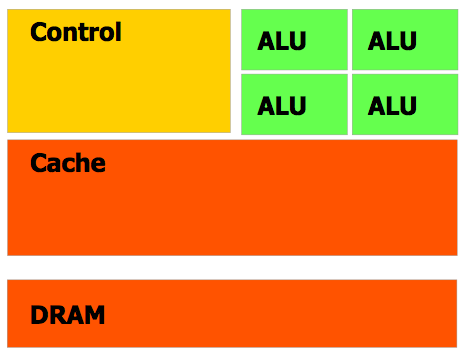
\includegraphics[width=0.8\textwidth]{Appendix/CPU}
\caption{CPU}
\label{fig:cpu_structure}
\end{subfigure}
\begin{subfigure}{0.50\textwidth}
\centering
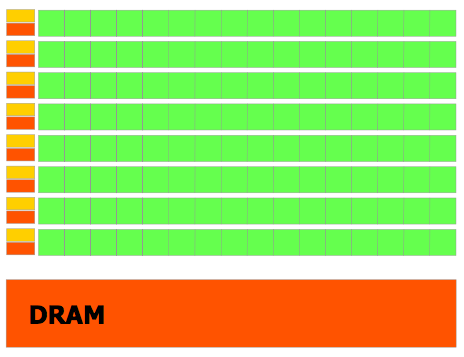
\includegraphics[width=0.8\textwidth]{Appendix/GPU}
\caption{GPU}
\label{fig:gpu_structure}
\end{subfigure}

\caption{Silicon Space Allocation (Taken from \cite[p.2]{cuda_doc})}
\label{fig:gpu_v_cpu}
\end{figure}

The key difference between \gls{cpu} and \gls{gpu} parallelism lies in the Flynn's taxonomy classification \cite{flynns_taxonomy} of architecture used by each.
\gls{cpu}s use a \gls{mimd} paradigm- this is parallelism of instruction as different \gls{cpu} cores can each be running different instructions concurrently.
Meanwhile, \gls{gpu}s use a \gls{simd} paradigm- this is parallelism of data as the same program is executed on a large quantity of data.
These differences can be most starkly visualised by observing the difference in the allocation of transistors between the two components (Fig. \ref{fig:gpu_v_cpu}). While the \gls{cpu} devotes a large amount of space to data caching and flow control, the \gls{gpu} allocates the vast majority of its capacity to data processing. \cite[p.2]{cuda_doc}

%briefly discuss jargon - device, host, etc.
%overview of the main differences:
%   parallelism of data vs parallelism of instruction
%compare speed ups that can be gained, reference Phil's project for more details

%MENTION DIFFICULTY GETTING ACCESS TO A GPU FOR TESTING:
Multiple \acrshort{cpu} cores are now commonplace in modern computers, including smartphones.
In contrast to this, dedicated \acrshort{gpu}s are normally only found in gaming PCs and consoles.
%This is changing, Apple now includes a custom \acrshort{gpu} in many of its mobile devices- metal?

\paragraph{\acrshort{cuda} vs OpenCL}
The two dominant languages for \gls{gpgpu} programming are \gls{cuda} and OpenCL, which were compared in detail by a previous project \cite{phil_diss}.
The key advantage that OpenCL has over \acrshort{cuda} is its portability.
Where \acrshort{cuda} is proprietary and runs only on NVIDIA hardware, OpenCL implementations are available for the majority of \gls{gpu} hardware including AMD, Apple \cite{apple_opencl}, Imagination and NVIDIA. \cite{opencl_conformance}
Nevertheless, this portability comes with a cost, code for different hardware must be tailored specifically to each hardware platform and performance has been shown to be consistently poorer \cite{cuda_v_opencl}.
The previous report also concluded that \gls{cuda} has better library support and is simpler to use \cite{phil_diss}.

%OpenCL runs on a wider number of devices, including mobile (iOS)
%frameworks, such as Apple's Metal allow significant simulations to be run, even on mobile devices

\section{Summary}
This chapter has reviewed the advantages and limitations of simulations as a replacement for \gls{in-vitro} experimentation.
It has assessed that the most significant limitation affecting the mass adoption of \gls{abm} \gls{in-silico} experimentation by biologists is the technical knowledge required to implement an efficient, parallel simulation.
Previous \gls{FLAME GPU} simulations have shown promise in their ability to run simulations on a standard desktop PC in comparable execution times to that of other simulations running on a high performance computing cluster \cite{flame_keratinocyte}.
The remainder of this project will further explore \gls{FLAME GPU}'s ability to help create fast simulations as well as the use of \gls{mde} to support the creation of these simulations.

\chapter{Tools and Platform}
\label{tools}

The remainder of this report explores the creation of a parallel \gls{FLAME GPU} implementation of the existing MASON \textit{PPSim} simulation.
The research focuses on ease-of-creation for parallel programs-- one of the key challenges outlined in Section \ref{ease-of-creation}.
The new simulation, \textit{PPSim v2}, still requires re-calibration and a comparison of results from a biological perspective which is clearly outside of the scope of this, a Computer Science project.

\section{Tools}
This project was developed on a machine running Ubuntu 16.04 with Intel i5 (650 @ 3.20 GHz) and 8GB of RAM.
The GPU utilised was an NVIDIA GeForce GTX 1050.
GPU programming utilised the latest version of \gls{cuda} (9.1).
\gls{cuda} was selected over OpenCL due to it being a requirement of \gls{FLAME GPU}.
Minimal knowledge of \gls{cuda} was needed for the development of the project as \gls{FLAME GPU} handles the majority of the \gls{gpu} hardware management.

In order to produce a working simulation of \gls{PP} formation, I have used an unreleased version (v1.5) of \gls{FLAME GPU}.
Amongst other features, \gls{FLAME GPU} v1.5 adds the ability to create agents from a host function between simulation steps.
As \gls{FLAME GPU} is developed openly, this version is freely available online \cite{flame_github}.
\gls{FLAME GPU} has been added to the project repository as a submodule, to ensure version compatibility between \gls{FLAME GPU} and \textit{PPSim v2}.

Eclipse Neon v4.6 and Epsilon v1.4 have been used with Java Runtime Environment 1.8.0 for developing the input XML model for \gls{FLAME GPU}.

Version-control for the simulation code, modelling tools and this report has been managed through Git and is available on \href{https://github.com/oliver-binns/PRIY.git}{GitHub}.
As this is an individual project, Git has been an acceptable solution.
If the scope of the project is to expand, it may become necessary to move the modelling section of the development into a more suitable version-control system, such as EMFStore\cite{emf_store} which is specifically designed for models.

%Approx 1500 words for problem description and analysis
\section{\gls{PP} Case Study}
\label{ppsim}
This project focuses on simulation as a tool for exploring biological systems at cell level.
This section is based on published research papers \cite{kieran_thesis, kieran_methodology, kieran_results, kieran_machine_learning, spartan} and discussion with \href{https://www.york.ac.uk/computational-immunology/members/kieran/}{K Alden}, who co-supervised the research for this project.
It uses an existing sequential \gls{MASON} simulation of \gls{PP} development \cite{kieran_thesis, kieran_methodology, spartan} (\textit{PPSim}) and attempts to use parallel computer architectures in order to speed this simulation up.

\textit{PPSim} has been used alongside \gls{in-vitro} lab experiments, and has contributed to new discoveries about the role of chemokines in PP development \cite{ppsim_findings, kieran_results}.
In achieving the biological results, each execution took \texttt{94.265} seconds, with \texttt{585,000} total executions being required for the statistical sampling technique being used.
The results were compiled using the York University High Performance Cluster, which is configured with 70 nodes, 138 processors, 1462 cores and 10.2TB RAM.
Even with a significant amount of \gls{cpu} parallelism available, the combined runtime of these executions is inconvenient and would be intractable for larger scale simulations \cite{kieran_machine_learning}.
As previously stated, \gls{FLAME GPU} can easily produce results to better a high-performance cluster, such as the one used to compute \textit{PPSim}, even on a standard desktop PC.
%Good, but give a PROBLEM DEFINITION
%WHAT HAS BEEN THE FOCUS OF THIS PROJECT?

\subsection{The \gls{domain}}
The domain model for \textit{PPSim} was developed according to the \acrshort{cosmos} process \cite{cosmos}, which was introduced in Section \ref{cosmos_intro}.
%Briefly detail how CoSMoS makes for better simulations
The model describes the cell behaviour over a 72 hour period in which \gls{PP}es develop.
\gls{PP}es are clusters of cells that form on the lining of the small intestine (Fig \ref{pp_imaging}).

\begin{figure}[htp]
\begin{subfigure}{0.70\textwidth}
\centering
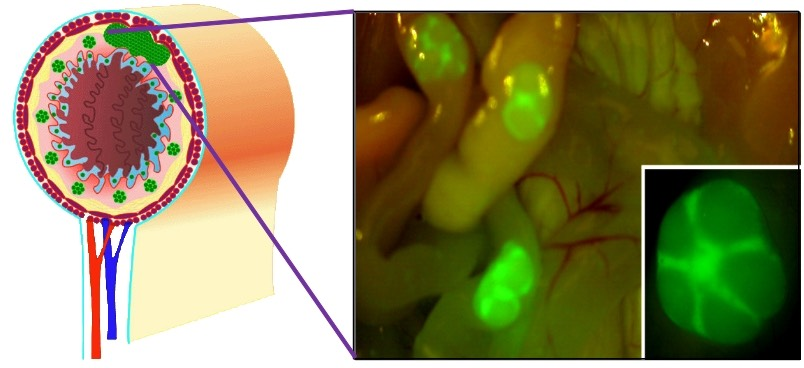
\includegraphics[width=\textwidth]{Appendix/Adult_PP}
\caption{Adult Peyer's Patch}
\label{fig:adult_pp}
\end{subfigure}
\begin{subfigure}{0.29\textwidth}
\centering
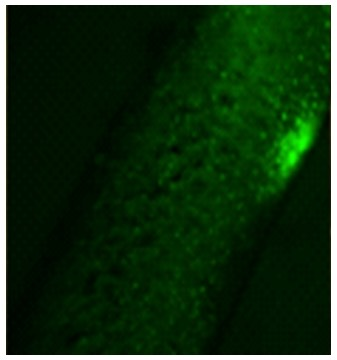
\includegraphics[width=\textwidth]{Appendix/Foetal_PP}
\caption{Foetal Peyer's Patch}
\label{fig:foetal_pp}
\end{subfigure}

\caption{Images of In-Vitro \gls{PP} (Provided by \href{mailto:mark.coles@york.ac.uk}{Mark Coles}, University of York)}
\label{pp_imaging}
\end{figure}

%ENVIRONMENT
In order to simulate \gls{PP}, a key design decision is to model the environment as a 3-dimensional tube but in 2-dimensions.
This is a reasonable abstraction to make as the cells move on the surface of the gut.
Agents leaving the environment in the x-direction are removed from the population and no longer considered.
Agents leaving the environment in the y-direction wrap around to the origin.

%AGENTS
In this model there are three types of agent which are all types of cells; \gls{LTo}, \gls{LTin} and \gls{LTi}.
State diagrams that describe the behaviour of each of these cells were presented as part of the original domain (Fig. \ref{fig:domain_state_diagrams}) and platform models (Fig. \ref{fig:platform_state_diagrams}) \cite{kieran_thesis}.

%Migration
The model starts when \gls{LTi} and \gls{LTin} cells begin migrating into the environment.
As such, at the beginning of the development process, neither of these cells are present.
\gls{LTi} and \gls{LTin} cells migrate into the environment throughout 72 hour time period being modelled.
%LTin
Initially these \gls{LTi} and \gls{LTin} cells move randomly around the environment.

%LTo
Stationary \gls{LTo} cells are randomly distributed around the environment.
These cells are present at the start of the development, but are dormant until an \gls{LTin} cell collides with them.
When this collision occurs, the \gls{LTin} may bind to the \gls{LTo} cell and the \gls{LTo} cell begins secreting a chemokine signalling protein.
Upon each addition \gls{LTin} collision, the \gls{LTo} starts to release chemokine at a greater rate.
Once the \gls{LTo} move into this new state, they will also divide every 12 hours, resulting in new \gls{LTo} cells.

%LTi
\gls{LTi} cells respond to the chemokine when the level in their local environment is great enough.
When this happens, they move towards the \gls{LTo} cell and eventually collide.
Upon collision \gls{LTin} cells may bind to the \gls{LTo} cell, as determined by the latter's adhesion level.
Neither \gls{LTin} and \gls{LTi} binds are permanent as the \gls{LTo}'s adhesion level may not be high enough to ensure prolonged contact.
Each successive contact with an \gls{LTin} cell increases the \gls{LTo}'s adhesion level, meaning that prolonged contact eventually becomes inevitable and the \gls{PP} is formed.

\section{The \gls{platform}}
\label{platform}
%platform-independent model
The platform model (Figs. \ref{fig:platform_state_diagrams} \& \ref{table:simulation_params}) refines the domain model and states how unknown or non-deterministic biological behaviour can be modelled \gls{in-silico}.
In particular, the platform model specifies models for adhesion between cells and how \gls{LTo} cells react to chemokine levels in their local environment \cite{kieran_thesis, kieran_methodology}.
One notable \textit{unknown} domain value is the rate that \gls{LTi} and \gls{LTin} cells y migrate into the environment.
In the \gls{platform} this is modelled at a constant rate, such that the \textit{known} correct number of cells is reached at the 12 hour time-step.

The platform model will be implemented using the \gls{FLAME GPU} framework.
This framework will be responsible for managing all data-structures and managing \gls{gpu} memory across different threads containing agent instances.

\section{Summary}
This chapter has summarised the tools used to implement the new parallel \textit{PPSim v2} simulation and outlined the biological background behind it.
\gls{FLAME GPU}, the simulation platform used for the new implementation uses X-machines \cite{xmachines} to define agents.
The existing \gls{domain} for \gls{PP} development is a good candidate for this new implementation as it already includes state models, which can be easily implemented as X-machines.

%Approx 2500 words for design and implementation
\chapter{Methods}
\label{methods}

%Intro Chapter:
The chapter details the simulation experiment that has been performed.
The experiment involved the development of a new \acrshort{gpu}-based \textit{PPSim v2} implementation as well as a new tool for mapping and transforming biological platform models into \gls{FLAME GPU} simulations.
Having previously established the current difficulties with biological simulation, this chapter also details how these are overcome in the implementation of this project.

\section{\gls{FLAME GPU} Simulation}
\label{ppsim_v2}
%HOW DOES THIS RELATE TO THE COSMOS PROCESS (ABOVE)
%platform-specific model
A \gls{FLAME GPU} implementation requires the creation of two artefacts (See Section \ref{flame_gpu}).
A structural `XML Model File' which defines the agents in the system and their allowed channels for communication.
A C source code file of `Scripted Behaviour' defines the actual behaviour of agents.

\subsection{Structural Model}
\gls{FLAME GPU} defines agents as X-machines in its XML model.
X-machines are structurally identical to finite state machines, other than that they have memory, which means it was possible to directly implement the platform model state diagrams directly into the \gls{FLAME GPU} simulation (Fig. \ref{fig:gmf_flame_generation}).

During the development of the model implementation, there were many occasions where the XML of the model because invalid because of human error.
These mistakes either caused ill-formed XML or an XML model which did not conform the \gls{FLAME GPU} model schema, which resulted in many tedious hours of debugging.
In order to mitigate the issues caused by these mistakes, a new tool was created using the Epsilon Modelling Framework.
The new tool ensures that any XML files that are created are valid XML and conform the the \gls{FLAME GPU} model schema.

In the tool, \gls{FLAME GPU} models can be designed using a graphical interface (Figs. \ref{fig:ltin_gmf} \& \ref{fig:ppsim_gmf}) and then exported to the required XML file format.
Adding this GUI front end to \gls{FLAME GPU} is a major step towards ensuring these parallel \gls{abm} simulations are more easily accessible by non-technical users.

\begin{figure}[htp]
\centering

\begin{subfigure}{0.49\textwidth}
\centering
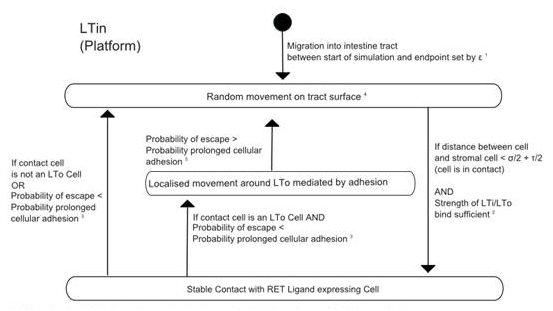
\includegraphics[width=\textwidth]{Appendix/Models/LTin_Cropped}
\caption{LTin Platform Model \cite{kieran_thesis}}
\label{fig:ltin_cropped}
\end{subfigure}
\begin{subfigure}{0.49\textwidth}
\centering
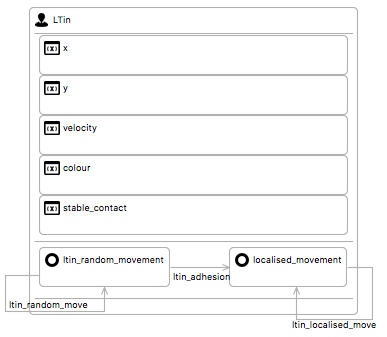
\includegraphics[width=0.7\textwidth]{Appendix/Models/LTin_GMF}
\caption{LTin Agent in Graphical Editor}
\label{fig:ltin_gmf}
\end{subfigure}

\begin{subfigure}{0.75\textwidth}
\centering
\begin{lstlisting}[language=XML, basicstyle=\tiny]
<gpu:xagent>
    <name>LTin</name>
    <description>Lymphoid Tissue initiator cell</description>
    <memory>
        <gpu:variable>
            <type>float</type>
            <name>x</name>
        ...
    </memory>
    <functions>
        <gpu:function>
            <name>ltin_random_move</name>
            <currentState>ltin_random_movement</currentState>
            <nextState>ltin_random_movement</nextState>
        ...
    </functions>
    <states>
        <gpu:state>
            <name>ltin_random_movement</name>
        </gpu:state>
        ...
        <initialState>ltin_random_movement</initialState>
    </states>
    <gpu:type>continuous</gpu:type>
    <gpu:bufferSize>5530</gpu:bufferSize>
</gpu:xagent>
\end{lstlisting}
\caption{\textit{Autogenerated} \gls{FLAME GPU} XML Model for LTin Agent}
\label{fig:xml_ltin}
\end{subfigure}

\caption{Autogeneration of \gls{FLAME GPU} Model File}
\label{fig:gmf_flame_generation}
\end{figure}
In addition to ensuring that only valid models can be produced, the graphical tool has a number of other benefits.
The original platform model (Fig. \ref{fig:ltin_cropped}) and the \gls{FLAME GPU} implementation (Fig. \ref{fig:ltin_gmf}) can now be compared at a glance.
For example, it is immediately clear that the platform model has been refined to include only two states in the final implementation.
This is far less obvious when comparing the platform model (Fig. \ref{fig:ltin_cropped}) with the XML code (Fig. \ref{fig:xml_ltin}).
The removal of the `Stable Contact' state is logical- this state is instantaneous and immediately transitions into either localised movement or random movement, meaning its transitions can be merged into those which already exist between the other two states.
The behaviour still exactly matches the platform model.

%for each agent type in its implementation, these have been directly implemented into it.
%A state-based platform model design is already available- the domain model for the original \gls{MASON} implementation of this simulation.
A number of other deviations were made from the platform model, mainly because of the time limitations of the project.
The decision to only include a single central \gls{LTo} cell in the simulation meant that the `No Expression of RET-Ligand' state could be removed, as it cannot be reached.

\label{missing_link}
Both the domain and platform model diagrams for \gls{LTi} cells are missing a transition from the `random movement' to `contact' state.
This is because \gls{LTi} cells may collide with \gls{LTo} cells, without having reacted to chemokine emission.
This transition was present into the original \gls{MASON} implementation of \textit{PPSim}, but was never corrected in the state diagram \footnote{Personal communication, \href{https://www.york.ac.uk/computational-immunology/members/kieran/}{K. Alden}}.
It has also been added into the new \gls{FLAME GPU} implementation.

\subsection{Behavioural Model}
The agent behaviour is defined in a \gls{cuda} source code file.
Code may be run on the \gls{Host} between simulation steps, or on the \gls{Device} during steps.
\gls{Host} functions have been used scarcely for minor administrative tasks, as they carry a data transfer penalty and do not benefit from \gls{gpu} parallelism.

The only two tasks handled by the \gls{Host} are tracking the current simulation time (by incrementing \texttt{SIM\_STEP} between each step) and managing the migration of cells into the environment.
The ability to create agents from a host function is currently only available in a pre-release version of \gls{FLAME GPU}, which is why this version of the software was selected.
Previously, agents could only be created during the simulation by other existing agents.
Creating another agent type solely to manage \gls{LTo} and \gls{LTin} migration would needlessly complicate our platform model, which is highly undesirable.
Furthermore, this implementation is very unintuitive and thus conflicts with our aim of simulations being simple to create.

%Host cell creation into the system is a work in progress for next \gls{FLAME GPU} release?
%Again, this is IMPLEMENTATION:
\gls{LTo} cells divide every 12 hours once they reach the `Upregulation of Chemokines' state.
A previous project on this topic stated that \gls{LTo} cell division must be performed sequentially on a host function in order to prevent new cells occupying the same space \cite{phil_diss}.
However, by adding a force resolution step, as used in previous \gls{FLAME GPU} simulations \cite{flame_keratinocyte}, this has been implemented in parallel, on the device.
As well as the speed up from parallelising the division step, implementing the feature in this way has also removed the cost of data transfer between the \gls{Device} and \gls{Host}.
%HACKY CELL DIVISION

Due to limitations of the \gls{FLAME GPU} framework and the time constraints on the project, there are several features of the \gls{platform} which I have not been able to implement.
Firstly, in this implementation the environment is static and does not grow.
Environmental growth would not be technically challenging to implement in \gls{FLAME GPU}.
A \gls{Host} function would increment the environment size variables at each time step, and transitions on each agent would allow them to adjust their positions accordingly the new size, in parallel.
However, due to \gls{FLAME GPU}'s dependence on state machines, this transition would have to be present on every state for every agent, and thus would be very time-consuming to implement.
On top of this, in the current version of \gls{FLAME GPU}, these transitions, which would be identical for every state of each agent, would be classed as different functions, and thus each implemented sequentially.
This would significantly increase the runtime of the simulation.
%can I state this?:
The original \textit{PPSim} produced the same statistical analysis results of with and without environmental growth\footnote{Personal communication, \href{https://www.york.ac.uk/computational-immunology/members/kieran/}{K. Alden}}, therefore the impact of this on the emergent behaviour is likely minimal.

Secondly, once \gls{LTo} cells transition into their `mature' state, they no longer divide.
%May result in a smaller PP, but unlikely to have *significant effect*
%Is this it?

\subsection{Execution}
\subsubsection{Initialisation}
\gls{FLAME GPU} simulations are initialised using another XML file specifying which, if any, agents are present at the beginning of the execution.
In this platform model there is a single \textit{active} \gls{LTo} cell in the centre of the environment.
%cite for WHY single, WHEN was this done before?

When in visualisation mode, the view is centred on the middle of the environment, with the environment bounds calculated from the position of the initial agents.
In order to ensure that these bounds are calculated correctly, the simulation is initialised using an \gls{LTi} cell placed at the maximum bounds of the environment (\texttt{7303}, \texttt{254}).
This single \gls{LTi} cell will have minimal impact on the overall simulation behaviour.

\subsubsection{Testing}
In order to obtain a fair representation of runtime, the simulation was executed as a console application \texttt{500} times, the same number of runs that was used for each parameter set of the MASON \textit{PPSim} implementation.
The simulation was run for its full length of \texttt{4321} steps (representing 72 hours).

As the new simulation is a re-engineering of the existing PPSim, it could inherit the validation of the existing simulation.
This requires the new simulation to be demonstrably similar with similar components, behaviours and results.
We can only assert that this is true to a certain extent.
The simulation itself is based on the same platform model and thus models the same biological components and behaviours.
However, due to the differences in implementation platform, the similarities in components do not extend down to the code level.

A full biological comparison is outside the scope for this project, therefore \textit{PPSim v2} will only be tested for face validity against its \gls{domain}.
A model has face validity if it demonstrates reasonable output \cite{model_validity}.
In this case, the simulation was expected to demonstrate a reasonable representation of the development of a \gls{PP} by the mechanisms described in Section \ref{ppsim}.

\section{Graphical Modelling Tool}
In order to implement a tool to support my \gls{FLAME GPU} development, the Epsilon Modelling Framework was selected.
The decision to use this framework was simple, as it provides all the tools required and I was already familiar with it.
The aim was for the tool to \textit{directly} map the platform model structures into the required \gls{FLAME GPU} XML model.
This should significantly improve the model design experience and allow for domain experts to be kept more involved with the simulation creation.
This new process is shown as part of the \gls{cosmos} process in Fig. \ref{fig:flame_improved}.

\begin{figure}[htp]
\centering
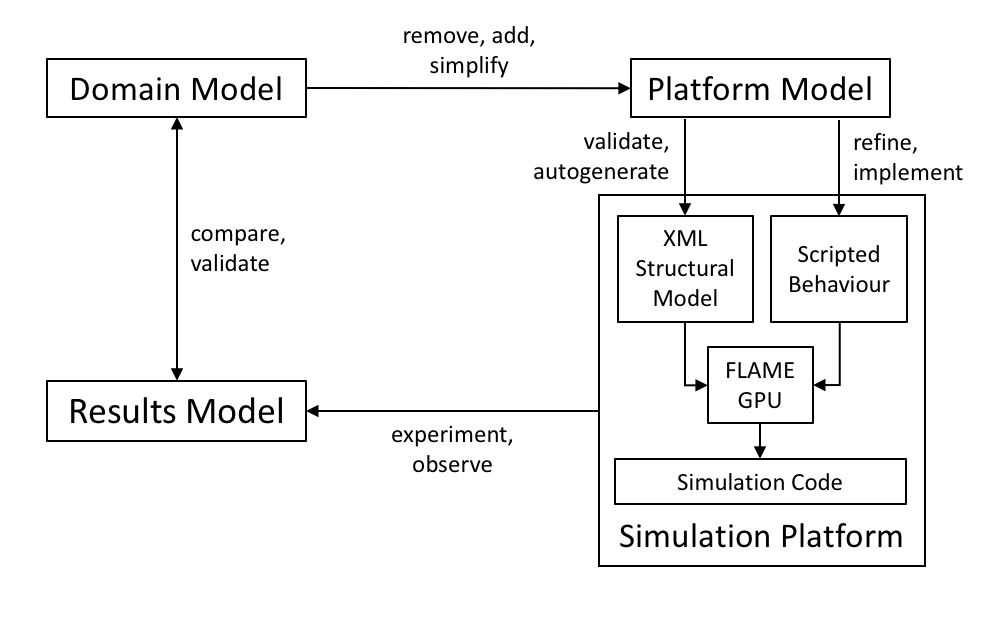
\includegraphics[width=0.7\textwidth]{Appendix/CoSMoS_FLAME}
\caption{Autogeneration of \gls{FLAME GPU} Artefact as part of the \gls{cosmos} Development Process-- See Fig. \ref{fig:cosmos_process}}
\label{fig:flame_improved}
\end{figure}

In this section, the underpinnings of the new graphical input for \gls{FLAME GPU} are outlined.
To design a graphical language in Epsilon, first a metamodel for the language is defined.
Then additional Epsilon tools are used to validate user inputs, and implement a model transformation from the new graphical model to the existing \gls{FLAME GPU} Model XML schema.
The full XML model used for the final simulation was automatically generated from a diagram model created within this graphical editor (Fig. \ref{fig:ppsim_gmf}).

\subsection{Metamodel}
A metamodel is required to formalise how models can be represented in our graphical modelling tool.
The development of the metamodel was guided by the existing \gls{FLAME GPU} XML model schema.
This model schema is itself a metamodel for the \gls{FLAME GPU} model file.
The new metamodel (See Section \ref{fig:gmf_metamodel}) was created using the Emfatic language, a convenience textual syntax for Ecore.
This Emfatic text can be used to generate an Ecore model which, in turn, is used to generate the GMF Graphical Editor.

%similarities:
%top level simulation contains:
%   variables
Much of the new metamodel matches the \gls{FLAME GPU} schema.
There is a top level simulation object which contains a list of agents, a list of messages that agents can send, etc.
One notable difference here, is that as simulations contain exactly one environment, the data contained in this tag (constants, step functions, etc.) is stored at the simulation level, and no Environment class exists.
The main difference in the new metamodel is its ability to utilise references to objects.
Using references to objects ensures that the objects being referred to exist, which must be the case for model to be valid.
For instance, we do not want to allow an agent to have an initial state that does not exist, setting this attribute as a reference in the metamodel ensures that this is not the case.

Due to the time constraints on this project, this metamodel is not quite a complete mapping to every \gls{FLAME GPU} feature.
Global Function Conditions, which act as a condition to determine whether a function should be applied to either all or none of the agents within a particular state, have not implemented.
Additionally, global variable arrays cannot be created using the tool, these variables may only be of type int, float or double.
Neither of these unimplemented features were required in the development of \textit{PPSim v2}.

\subsection{EuGENia}
A GMF editor was created by adding EuGENia annotations into the Emfatic metamodel.
These annotations are used to automatically generate the \texttt{.gmfgraph}, \texttt{.gmftool} and \texttt{.gmfmap} models required for the GMF Graphical Editor.
EuGENiA provide a flexible range of options for displaying model data in different ways in the graphical editor \cite{epsilon_book}.
Implementing the graphical editor required a number of important decisions here, in order for the tool to provide a logical user experience to modellers.

The majority of the graphical editor design was straightforward, with top level items such as agents, global variables and messages being displayed as nodes on the diagram.
Variables and states that belong to agents are displayed as inner nodes in containers within these nodes.
EuGENiA allows transitions between states to be displayed as directional links, meaning the state diagrams for each agent can be displayed in the same way as they appear on the domain diagram (Fig. \ref{fig:ltin_gmf}).

A number of implementations for transition conditions were considered during development.
Due to the limitations in the GMF Graphical Editor, values under containment cannot be edited unless they are displayed on the diagram.
For obvious reasons, the transitions which are displayed as links, cannot display nodes on the diagram inside them, or link to them.
In order to add edit the conditions on these transitions, the tree-based editor was used.
This was recommended as the simplest approach by the lead developer of Epsilon team\footnote{Personal communication, \href{https://www-users.cs.york.ac.uk/dkolovos/}{D. Kolovos}}.
Other options that were considered include implementing the diagram as a Petri net where conditions are displayed as intermediary nodes in between two states.
With additional time, more sophisticated tools could allow a more elegant graphical editor to be produced.

\subsection{\acrfull{egl}}
\begin{wrapfigure}{r}{0.63\textwidth}
\centering
\begin{lstlisting}[language=XML, basicstyle=\tiny]
<states>
    [%for (state in agent.states){%]
    <gpu:state>
        <name>[%=state.name%]</name>
    </gpu:state>
    [%}%]
    <initialState>[%=agent.initialState.name%]</initialState>
</states>
\end{lstlisting}
\caption{Trivial Generation of \gls{FLAME GPU} XML Model}
\label{fig:egl_example}
\end{wrapfigure}

\gls{egl} was used to implement the transformation of the Epsilon GMF models into a \gls{FLAME GPU} XML model.
Since the tree structure of the GMF models already closely match the \gls{FLAME GPU} model schema, this process was trivial and simply involved adding in the required XML tags in between the model data and retrieving the correct identifiers for any object references.

\subsection{\acrfull{evl}}
The \gls{evl} has allowed well-formedness constraints to be implemented for the \gls{FLAME GPU} input model.
This should provide intuitive feedback (Fig. \ref{fig:validation_gmf}) in cases where the model may be incorrect, ensuring that all generated XML models conform to the \gls{FLAME GPU} input model schema.
Many of the \gls{evl} constraints have been used to cover shortcomings in the Ecore metamodel.
In particular, Ecore allows any attribute to be null, whereas in the majority of cases XML tags are not optional in \gls{FLAME GPU}.
Figs. \ref{fig:validation_gmf} \& \ref{fig:validation_quickfix_gmf} show how the \gls{evl} constraints would deal with a null initial state value for the \gls{LTin} agent.

\begin{figure}[htp]
\centering
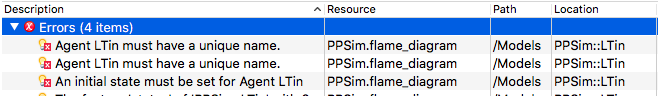
\includegraphics[width=\textwidth]{Appendix/validation_gmf}
\caption{Graphical validation using \gls{evl} constraints}
\label{fig:validation_gmf}
\end{figure}

As well preventing null values, preventing obviously nonsensical values has also been a key use for \gls{evl} constraints.
An example of this is ensuring that agents select one of their own states as their initial state, rather than one belonging to another agent.
This will help to reduce the number of model errors that reach the \gls{FLAME GPU} implementation stage.

%CRITIQUES ALSO USED?
%boolean transition conditions:
%critique allows users to ignore it
%BUT generally, and particularly with biological models like this:
%Transitions.. BETWEEN states require some form of external trigger?

\begin{figure}[htp]
\centering
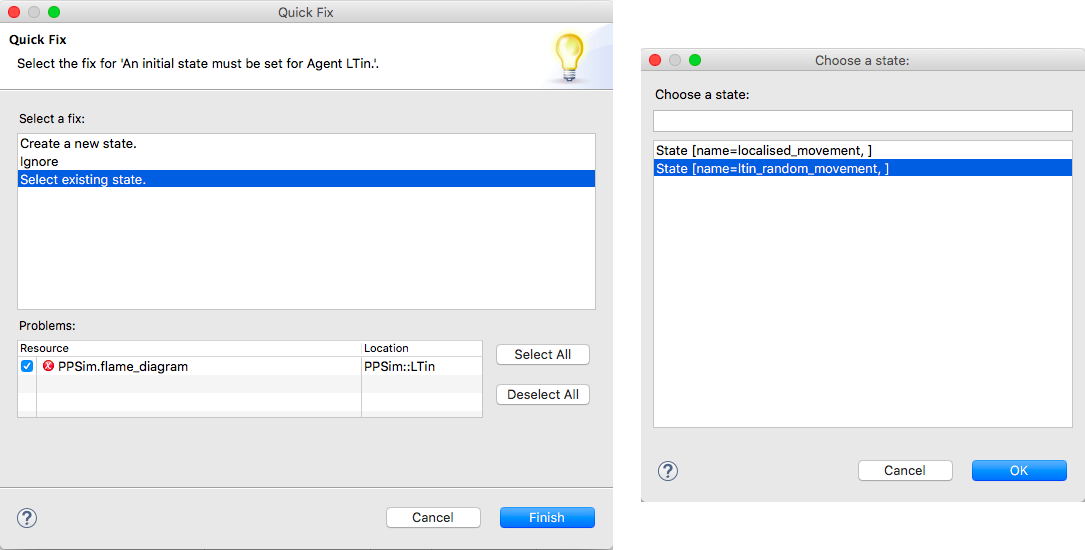
\includegraphics[width=\textwidth]{Appendix/validation_quickfix_gmf}
\caption{Quick fix of invalid model}
\label{fig:validation_quickfix_gmf}
\end{figure}

Quick fixes (Fig. \ref{fig:validation_quickfix_gmf}) have also been implemented to guide the user through easily correcting their invalid model.
The error feedback provided by these quick fixes is much more intuitive to non-technical users than that provided by \gls{FLAME GPU}.
%give example of FLAME GPU feedback

\section{Summary}
This chapter has described the implementation of a new \gls{FLAME GPU} simulation, \textit{PPSim v2}.
The \gls{mde} tools that have been developed to aid this implementation allow the simulation parameter values to be adjusted at will by non-technical users.
It has demonstrated proof-of-concept for automatically producing simulation artefacts from biological platform models and thus should allow future simulations to be implemented much more quickly.

%Approx 2500 words for results and evaluation
\chapter{Results}
\label{results}

\section{Ease of Creation}
The new Epsilon tool has shown that direct mappings from a biological platform model to a simulation code are possible.
Based on this, further work is now being developed with \href{http://paulrichmond.shef.ac.uk/gpu/gpucomputingatsheffield/}{Paul Richmond's \gls{FLAME GPU} group} at the University of Sheffield, to enhance the accessibility of \gls{FLAME GPU} for simulation developers (See Section \ref{flame_further_work}).
This should allow the simulation developer to focus ensuring domain details are correct, rather than battling the agent platform.
An improved version of this mapping, which abstracts away all \gls{FLAME GPU} implementation details such as partitioning, could bring additional benefits in this area, including ensuring that the simulation code always supports the latest hardware features.

\begin{figure}[htbp]
\begin{subfigure}{0.5\textwidth}
\begin{subfigure}{\textwidth}
\centering
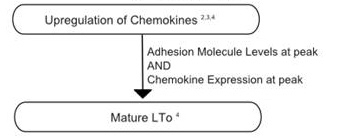
\includegraphics[width=\textwidth]{Appendix/LTo_Domain_Trace}
\caption{Section of \gls{domain} (See Fig. \ref{fig:domain_state_diagrams})}
\bigskip
\bigskip
\end{subfigure}

\begin{subfigure}{\textwidth}
\centering
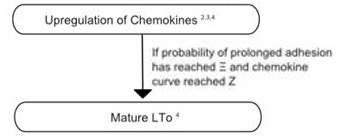
\includegraphics[width=\textwidth]{Appendix/LTo_Platform_Trace}
\caption{Section of \gls{platform} (See Fig. \ref{fig:platform_state_diagrams})}
\end{subfigure}

\end{subfigure}
\begin{subfigure}{0.5\textwidth}
\begin{lstlisting}[language=XML, basicstyle=\tiny]
<gpu:function>
    <name>mature</name>
    <currentState>chemokine_upregulation</currentState>
    <nextState>matured</nextState>
    <condition>
        <lhs><condition>
            <lhs>
                <value>CHEMO_LOWER_ADJUST</value>
            </lhs>
            <operator>==</operator>
            <rhs>
                <agentVariable>linear_adjust</agentVariable>
            </rhs>
        </condition></lhs>
        <operator>&amp;&amp;</operator>
        <rhs><condition>
            <lhs>
                <value>MAX_ADHESION_PROBABILITY</value>
            </lhs>
            <operator>==</operator>
            <rhs>
                <agentVariable>adhesion_probability</agentVariable>
            </rhs>
        </condition></rhs>
    </condition>
    ...
\end{lstlisting}
\caption{Fragment of \gls{FLAME GPU} Model}
\end{subfigure}
\caption{Traceability of \texttt{Mature} transition from \gls{domain} through \gls{FLAME GPU} Implementation}
\label{fig:traceability_condition}
\end{figure}

An additional benefit of this mapping, provides traceability from the domain model through to the simulation code.
This can be clearly seen in Fig. \ref{fig:traceability_condition}, which shows how the transition from `Upregulation of Chemokines' to `Mature \gls{LTo}' is refined from the \gls{domain} to \gls{platform} and then implemented in \gls{FLAME GPU}.
This traceability results in greater certainty that the simulation is faithful to the domain and no bugs have been produced during the implementation.

Furthermore, additional traceability helps to ensure that all artefacts contained in the domain model, platform model and simulation code are kept up-to-date with new information.
In Section \ref{missing_link}, a transition which was missing in the original domain and platform models was discussed.
In the new process, where \gls{FLAME GPU} model implementations are generated from the platform model, this transition could not be added into the implementation without first being added to the platform model.

This also tool aids development by finding and correcting model mistakes using \gls{evl}, this reduce the amount of time that developers spend debugging their code and increase productivity.
Clearly this shows that the new process could help to detect mistakes in both the domain and platform models.
\\\\
\textit{This work is ongoing.}

\section{Speed Up}
\subsection{Implementation Differences}
Unfortunately a number of differences between the \gls{MASON} and \gls{FLAME GPU} platforms have meant that it is not trivial to compare them.

\gls{FLAME GPU}'s use of Message Passing to send adhesion probabilities in parallel has given rise to the possibility of outdated variables.
In order to ensure maximum parallelism, the implementation used means that the probability of adhesion is the same for each collision that occurs in the same step of the simulation.
If multiple \gls{LTi} cells collide with an \gls{LTo} cell in the same step, the behaviour will be somewhat different to that of the \gls{MASON} implementation.
Before the next step, the adhesion probability emitted by the \gls{LTo} is updated for each collision, so the first collision of each step behaves the same as the \gls{MASON} implementation.
%is it ok to say this?
The impact of this is likely minimal as multiple collisions are unlikely to occur in the same timestep, due to the sparse population of the environment.

%WHY:
As well as differences in the implementation, including the use of message passing and force resolution used for \gls{LTo} cell division, the results have also been gathered using different hardware.
This is obvious, as the implementations have different hardware requirements.
The original \gls{MASON} \textit{PPSim} simulation works well when executions can be run in parallel across multiple \gls{cpu} processors.
The new \textit{PPSim v2} implementation requires NVIDIA \gls{gpu} hardware, which is not commonly available.
The combined effect of these differences makes the initial hypothesis, of the two platform implementations being comparable, untenable.

Within the scope of a Computer Science Masters' Degree project it has not been possible to replicate all the activities of the original \textit{PPSim} development.
In particular, future work on this simulation will need to rerun simulation calibration, sensitivity analysis and the bio-comparable experimentation \cite{kieran_thesis, kieran_results}.

\subsection{Comparison}
%SPEED RESULTS..
Instead, a new hypothesis is that the platform model for the \gls{FLAME GPU} implementation is comparable to the original biological model.
If our new platform model can be shown to be refined from the original PPSim domain model, we can say that this simulation also shows Peyer's Patch development, and thus is a faster representation of this biological process.
The only concern addressed in this report is that of face validity of the simulation.
Further biological comparisons still need to be performed.
%Pragmatically, it makes more sense to compare this implementation to its original domain, as this is the entire aim of the process?

In order to test this hypothesis, we will ensure that the following emergent behaviour is reasonable, and similar to the \gls{domain}:
\begin{itemize}
    \item Initialisation of the simulation with single central \gls{LTo} cell
    \item \gls{LTi}(n) cells migrate into the gut at a constant rate and move randomly
    \item \gls{LTo} begin to attract \gls{LTi} cells after any collision from \gls{LTin} cell
    \item \gls{PP} cell cluster forms around the original \gls{LTo} cell before the end of the simulation
\end{itemize}

\gls{FLAME GPU} provides a visualisation which can be used to demonstrate the appearance of the expected emergent behaviour.
This behaviour appears to be present, and reasonable, in the \textit{PPSim v2} simulation, as shown by Fig. \ref{fig:ppsimv2_vis}, however this has not been verified by a domain expert.
\newpage
\begin{figure}[htpb]
\begin{subfigure}{\textwidth}
\centering
\frame{
\includegraphics[width=\textwidth]{Appendix/Sim/Start}}
\caption{Beginning of simulation, single central \gls{LTo} cell is present.}
\label{fig:sim_start}
\end{subfigure}
%\end{figure}

%\newpage

%\begin{figure}[htpb]\ContinuedFloat
\begin{subfigure}{\textwidth}
\centering
\frame{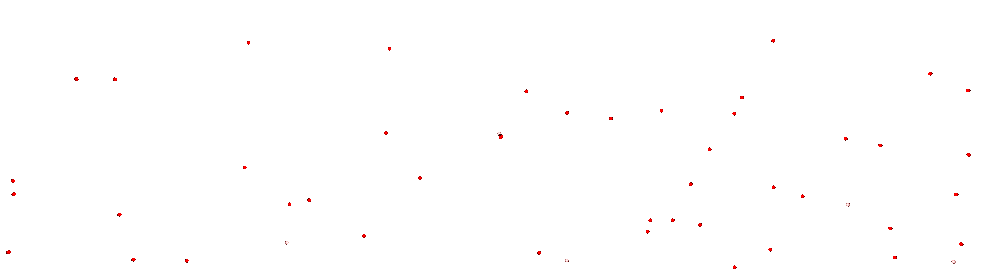
\includegraphics[width=\textwidth]{Appendix/Sim/Migration}}
\caption{\gls{LTin} \& \gls{LTi} cells migrate into the environment and activate \gls{LTo} cell.}
\label{fig:sim_contact}
\end{subfigure}
%\end{figure}

%\begin{figure}[htpb]\ContinuedFloat
\begin{subfigure}{\textwidth}
\centering
\frame{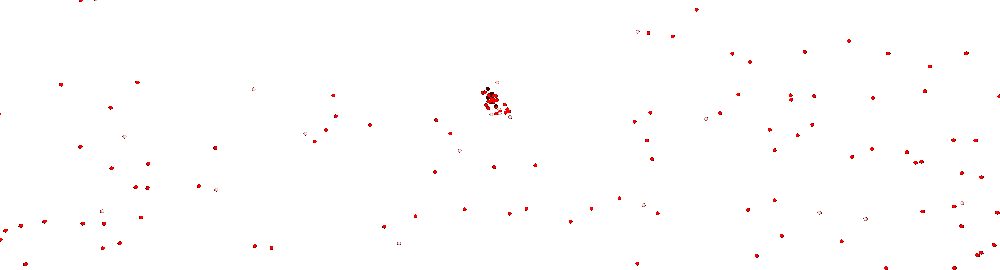
\includegraphics[width=\textwidth]{Appendix/Sim/Patch}}
\caption{Chemokine emission \& \gls{LTo} cell division causes \gls{PP} to form.}
\label{fig:sim_patch}
\end{subfigure}

\caption{Visualisation of \textit{PPSim v2} produced using \gls{FLAME GPU}}
\label{fig:ppsimv2_vis}
\end{figure}

As the simulation is \gls{gpu}-based, the visualisation has minimal impact on the run-time of the new simulation.
The new version of the simulation, \textit{PPSim v2}, has an average runtime of \texttt{35.828} seconds over \texttt{500} console-only executions.
This runtime can be reduced drastically to only \texttt{25.039} seconds when XML output is turned off, due to the large cost of data-transfer between the \gls{gpu} and its \gls{Host}.
These runtimes are both significantly less that the \texttt{94.265} seconds proffered by the original \gls{MASON} \textit{PPSim}.
Nevertheless, the aforementioned differences in the model implementations means that further biological analysis must fully validate \textit{PPSim v2} against the \gls{domain} before the results can be wholly accepted.
%different hardware

%Approx 1000 words
\chapter{Conclusion}
%NB.. INTRODUCTION + CONCLUSION MUST MATCH AND REFERENCE EACH OTHER.
This project began with an ambitious set of goals, stated in Section \ref{aims}.
%Review of the use of simulations, with a particular focus on computational biology. This review should explore the advantages that in-silico testing provides over in-vitro experimentation and the problems that must be overcome for the mass adoption of biological simulations.
Over the course of the project, the use of simulations as well as its advantages over \gls{in-vitro} experimentation has been reviewed.
The biggest problems affecting the adoption of \gls{abm} simulations have been identified.
Most significantly is that fast simulations of complex models are far too difficult to create, meaning experienced software developers are required.
This has fulfilled our Aim 3.

%Explore the findings of the new implementation and discuss how these can be generalised between different simulations.
The new implementation has shown that cell division \textit{can be generalised between different simulations}.
Other general features such as random cell movement has been discussed as another suitable candidate for generalisation.
This has met and exceeded this part of the original aim.

%   Discuss techniques for allowing non-technical users to easily create formal models that can be transformed into new simulation implementations.
\gls{mde} has been proposed as a \textit{[technique] for allowing non-technical users to easily create formal models that can be transformed into new simulation implementations}.
The \gls{mde} approach, taken in this project, has already realised numerous benefits in this area.
The new graphical tool allows non-technical users to easily transform parts of \textit{existing} platform models into \gls{FLAME GPU} structural models.
The reuse of artefacts is a fundamental part of \gls{mde}.
This has given domain experts the ability to modify key simulation parameters, such as the sizes of cells and cell input rates.
This ability is very useful for experimentation and for refining the simulation if new biological knowledge is discovered.
The adjusted parameters can be automatically realised in the simulation code, something which would have previously required a software developer.
%significant resources, but MDE gains not normally realised until tool/model reuse
%Establish a firm grounding for the future development of new tools to allow fast, parallel simulations of biological systems to be easily created by non-technical users.
This is a \textit{firm grounding for the future development of new tools} that will allow non-technical users to easily create fast, parallel simulations of biological systems.

%Develop a parallel implementation of an existing sequential simulation of Peyer’s Patch development and explore any speed increases that can be produced using General Purpose GPU programming (GPGPU) programming.
An initial aim of this project was \textit{`to explore the speed increases that can be produced by using \gls{gpgpu} programming'}.
A simulation has been created that displays the formation of \gls{PP}es, and while this has been shown to execute in less time that the original sequential \textit{PPSim} there are too many differences in their implementations to directly compare them.
The runtime of \textit{PPSim v2} is still likely to be inconvenient if a great number of runs is needed.
A sensible approach could be to use this faster simulation to generate training data for the machine learning approach described in \cite{kieran_machine_learning}.
Alternatively, a further level of parallelism, where different executions are run across multiple \gls{gpu}s could be a way to ensure a more realistic total runtime.

In conclusion, the goal of recreating \textit{PPSim} has been partly achieved: a working simulation exists and it recreates the basic visual behaviour of \textit{PPSim}. 
The goal of ensuring parallel simulations are easier to create has been demonstrated, by capturing the inherent metamodel of the \gls{FLAME GPU} input language (XML) and developing a graphical tool for producing new models.
The project provides a well-engineered and documented basis for further work on the efficient engineering of parallel simulations in \gls{FLAME GPU}\footnote{Personal communication, \href{http://www.scm.keele.ac.uk/staff/f_polack/}{F. Polack}, \href{https://www.york.ac.uk/computational-immunology/members/kieran/}{K. Alden}, co-supervisors}.

\section{Further Work}
\subsection{Peyer's Patch Case Study}
Although the two \gls{PP} simulations are both derived from the same domain model, implementation differences between them mean they are not yet fully comparable.
While the different computational platforms may ultimately limit a full comparison, the long-term goal is to replace the MASON implementation of \textit{PPSim} with the new \gls{FLAME GPU} \textit{PPSim v2} so as to increase the possible biological use-cases of the simulation.
Future work will need to explore the meaning of the implementation differences between simulations and whether that have any effect on their validity against the domain model.

Further work on this topic is needed to show that these implementations can still produce results in an acceptable time when scaled up.
With this simulation in particular some options for increasing the scale include modelling in 3-dimensions, adding further cell types and biological factors and cell types into the model, and simulating the whole length of the gut rather than a small section.

\gls{FLAME GPU} provides some tips for ensuring that simulations are as efficient as possible\cite[p.37]{flame_doc}.
In particular, the tips state that populations with low numbers (such as \gls{LTo} cells in \textit{PPSim v2}) will perform poorly.
For populations of agents less than 2000, non-partitioned messages have less overhead than spatial partitioning.
Due to the initially empty environment and gradual entry of \gls{LTin} and \gls{LTi} cells, for much of the \textit{PPSim v2}, this is the case.
Different variations of the tips could be explored further with the intention of driving further performance improvements into \textit{PPSim v2}.

%SPARTAN?
%can we produce any new hypotheses from this?
Spartan is a tool for understanding relationships and providing novel biological insight into simulation behaviour.
Spartan was use for analysing the results of the original PPSim implementation \cite{spartan} and may provide an insight into validity of the parallel \textit{PPSim v2} implementation.

\subsection{\gls{FLAME GPU}}
\label{flame_further_work}
A number of enhancements to the open-source \gls{FLAME GPU} framework would have made the implementation of \textit{PPSim v2} easier to create and faster to run.
This further work section is being discussed with \href{http://paulrichmond.shef.ac.uk/gpu/gpucomputingatsheffield/}{Paul Richmond's \gls{FLAME GPU} group} at the University of Sheffield, however as \gls{FLAME GPU} is open-source, these enhancements could also be made by members outside the group.

Firstly, a method to implement global agent `step' functions, that is to say, functions which are applied to every agent of a particular type, regardless of their current state.
This would allow the environmental growth feature to be easily implemented, with a global step function used to update agent positions as the environment grows.

%parallel layer functions
Currently each distinct agent transition function is run sequentially, despite \gls{FLAME GPU} providing "functions layers" as a mechanism to define which of these transitions can be run in parallel.
Future improvements to \gls{FLAME GPU} should run these transitions in parallel using the new NVIDIA hardware feature--  multiple \acrshort{cuda} cores.
This should have a measurable positive impact on existing \gls{FLAME GPU} simulations.

%cell division, stop hacky: force resolution, etc.
%while TRUE resolve..

\subsection{Software Generalisibility}%IS THIS A WORD?
%Expand project for more powerful cell based simulation
%allow access to non-technical users
%flexible modelling
While the use of Epsilon has allowed for domain experts to be kept involved with the model implementation, there is still a final, most technically challenging, stage of the simulation creation where the agent behaviour is programmed.
Further work will need to study general agent behaviour in these forms of biological simulation.
The reuse of a previous simulation's implementation of cell division behaviour, has shown that at least some behaviour is common across different simulations.
The power of \gls{mde} is such that this repeated behaviour should be generalised to reduce the time needed and prevent the mistakes that occur during reimplementation of the similar software features.
%FUTURE WORK is needed to provide the ability to modify agent behaviour

On top of this, with the current implementation, technical platform-specific implementation details (layer functions and agent partitioning) have become part of the model.
Ideally these should be extracted from the model implementation and automated.

\subsection{Hardware Availability}
%Talk about difficulty getting access to the necessary NVIDIA hardware
One of the greatest challenges of this project has been gaining access to NVIDIA GPU hardware.
While these are available off the shelf in most high-street computer retailers, they are not commonly found as part of standard desktop PCs, which generally contain integrated graphics hardware.
Indeed, none of the software lab PCs at the University of York contain the dedicated graphics chips required to run this software.
Future work could re-evaluate whether the benefit of a cross-platform API, such as OpenCL, could outweigh the performance benefit provided by \acrshort{cuda}.
%OpenCL could be something to discuss here
%dismissed by Phil, but further exploration could be good!
%ANDY is working on this

\printbibliography

\appendix
\chapter{\textit{PPSIM V2} COMPONENTS}

Other supplementary material, including \gls{FLAME GPU} simulation code is available in the project \href{https://www.github.com/oliver-binns/PRIY.git}{GitHub repository}.

\begin{figure}[htp]
\centering
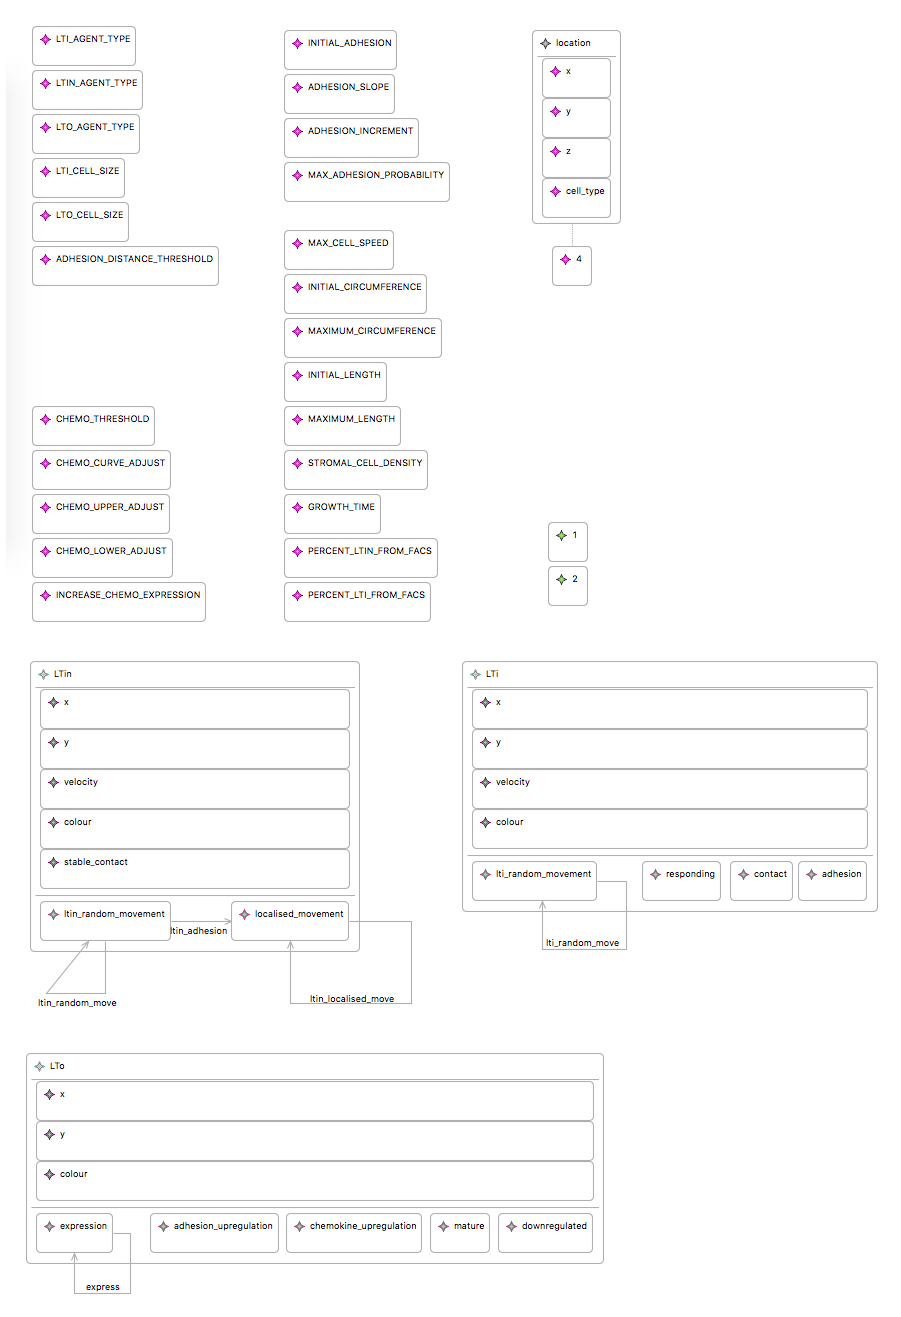
\includegraphics[width=\textwidth]{Appendix/ppsim_gmf}
\caption{Graphically produced \gls{FLAME GPU} Simulation model for Peyer's Patch}
\label{fig:ppsim_gmf}
\end{figure}

\newpage

\section{Metamodel for Graphical Editor}
\label{fig:gmf_metamodel}
\lstinputlisting[language=Java, basicstyle=\tiny]{../Epsilon/Metamodels/Metamodel.emf}

%\section{Generated FLAME GPU Model}
%\label{fig:flame_model}
%\lstinputlisting[language=XML, basicstyle=\tiny]{../FlameGPU/src/model/XMLModelFile.xml}

%\section{FLAME GPU Behaviour Script}
%\label{fig:flame_behaviour}
%\lstinputlisting[language=XML, basicstyle=\tiny]{../FlameGPU/src/model/functions.c}

\chapter{DOMAIN \& PLATFORM MODEL DIAGRAMS}

\begin{figure}[htp]
\centering
\begin{subfigure}{0.95\textwidth}
\centering
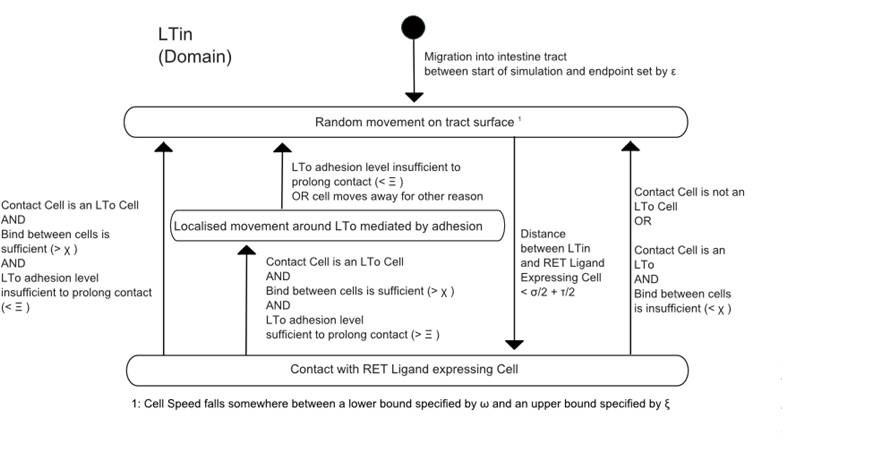
\includegraphics[width=\textwidth]{Appendix/Models/Domain/LTin}
\caption{LTin}
\end{subfigure}
\end{figure}

\begin{figure}[htp]\ContinuedFloat
\centering
\begin{subfigure}{0.95\textwidth}
\centering
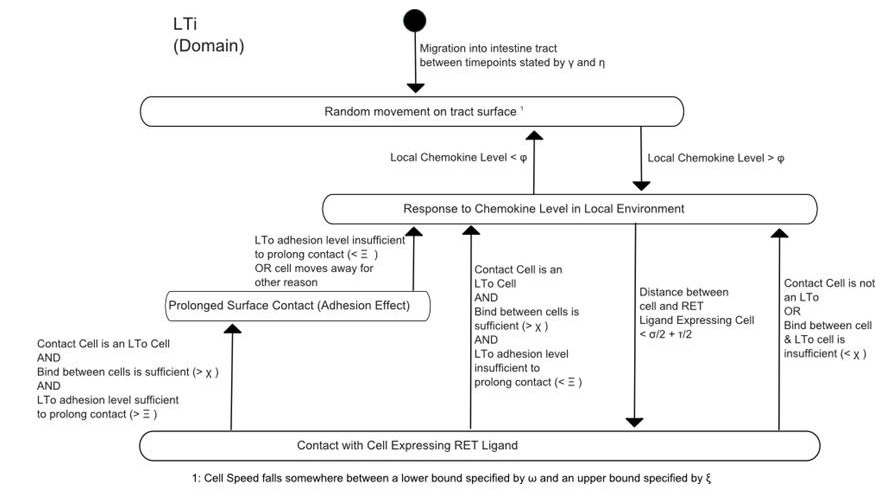
\includegraphics[width=\textwidth]{Appendix/Models/Domain/LTi}
\caption{LTi}
\end{subfigure}
\end{figure}

\begin{figure}[htp]\ContinuedFloat
\centering
\begin{subfigure}{0.95\textwidth}
\centering
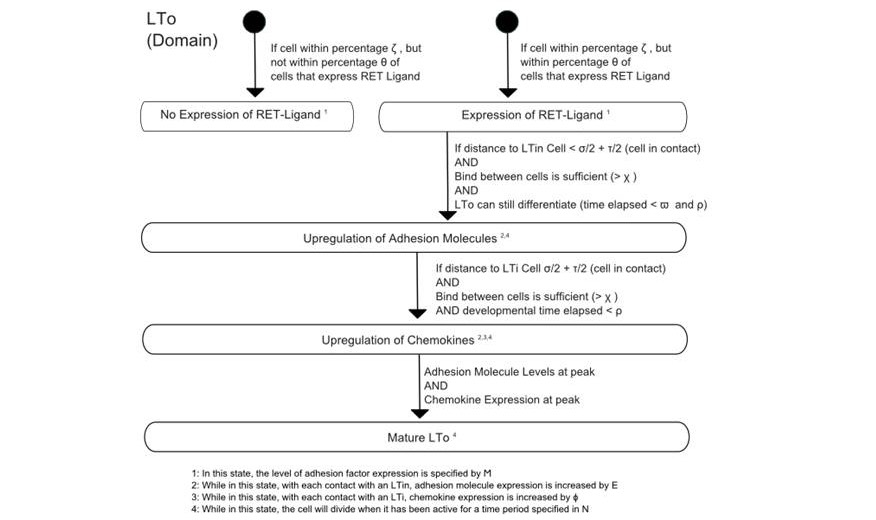
\includegraphics[width=\textwidth]{Appendix/Models/Domain/LTo}
\caption{LTo}
\end{subfigure}

\caption{Domain Model State Diagrams \cite{kieran_thesis, kieran_methodology}}
\label{fig:domain_state_diagrams}
\end{figure}

\begin{figure}[htp]

\begin{adjustbox}{center}
\begin{tabular}{|c|l|r|} 
\hline
& Parameter & Value \\
\hline
\textchi & Probability stable bind occurs on contact & 50\% \\ 
\texttheta & Percentage of \gls{LTo} cells expressing RET Ligand & \textit{Unknown} \\ 
\textEta & Percentage of RET Ligand Cells that are non-stromal & \textit{Unknown} \\ 
$\varpi$ & Hours Immature \gls{LTo} remains active & 72 hours \\ 
\textNu & \gls{LTo} Division Time & 12 hours \\ 
\textrho & Hours RET Ligands Expressed & 72 hours \\ 
\texttau & \gls{LTin} / \gls{LTi} Cell Size & 8 \textmu m \\ 
\textsigma & \gls{LTo} Cell Size & 24 \textmu m \\ 
\textomega & \gls{LTin} / \gls{LTi} Speed Lower Bound & 3.8 \textmu m / min \\ 
\textxi & \gls{LTin} / \gls{LTi} Speed Upper Bound & 8.8 \textmu m / min \\ 
\textepsilon & \gls{LTin} Input Time & 72 hours \\ 
\textgamma & \gls{LTi} Input Delay Time & 0 hours \\ 
\texteta & \gls{LTi} Input Time & 0 hours \\ 
\textphi & Chemokine Threshold & \textit{Unknown} \\ 
\hline
\end{tabular}
\end{adjustbox}

\caption{Domain Model Biological Parameters \cite{kieran_thesis, kieran_methodology}}
\label{table:domain_params}
\end{figure}

\begin{figure}[htp]
\centering
\begin{subfigure}{0.95\textwidth}
\centering
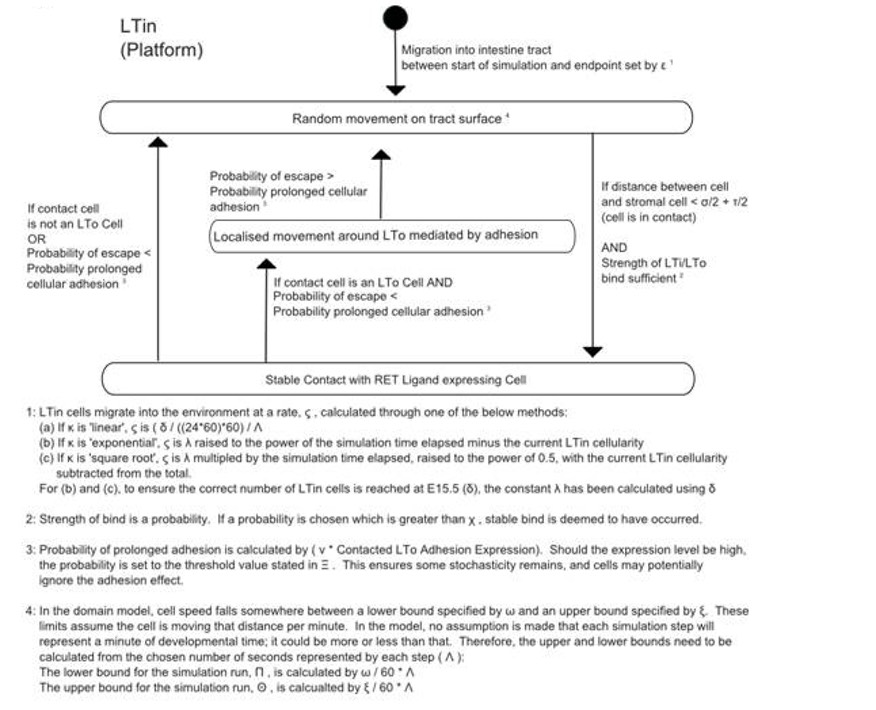
\includegraphics[width=\textwidth]{Appendix/Models/Platform/LTin}
\caption{LTin}
\end{subfigure}
\end{figure}

\begin{figure}[htp]\ContinuedFloat
\centering
\begin{subfigure}{0.95\textwidth}
\centering
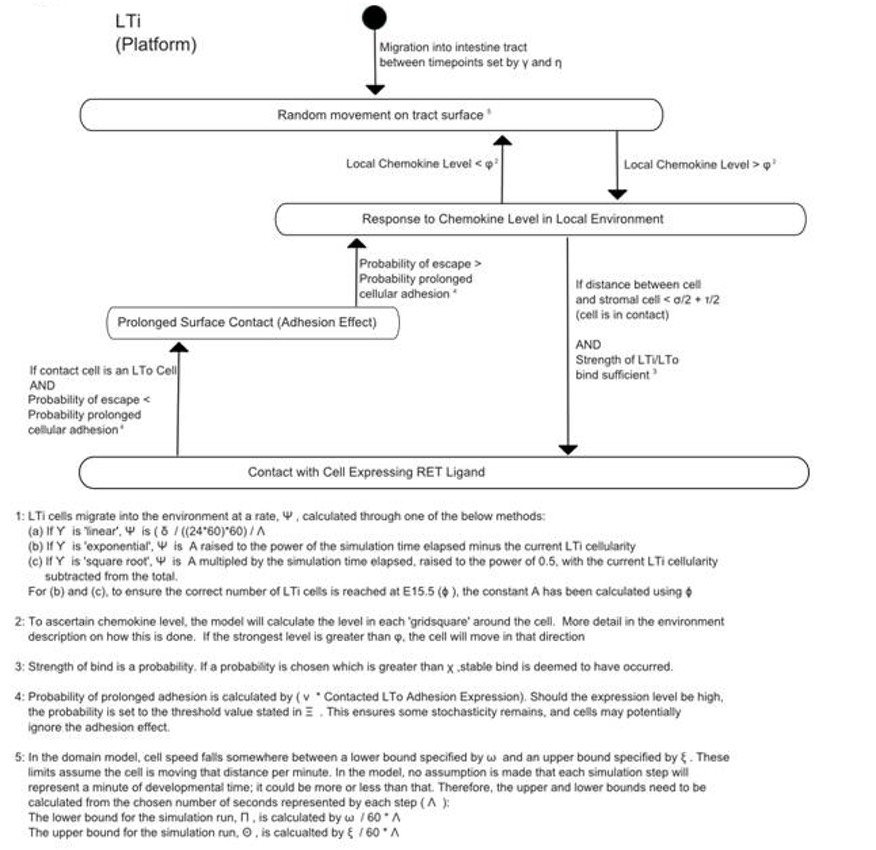
\includegraphics[width=\textwidth]{Appendix/Models/Platform/LTi}
\caption{LTi}
\end{subfigure}
\end{figure}

\begin{figure}[htp]\ContinuedFloat
\centering
\begin{subfigure}{0.95\textwidth}
\centering
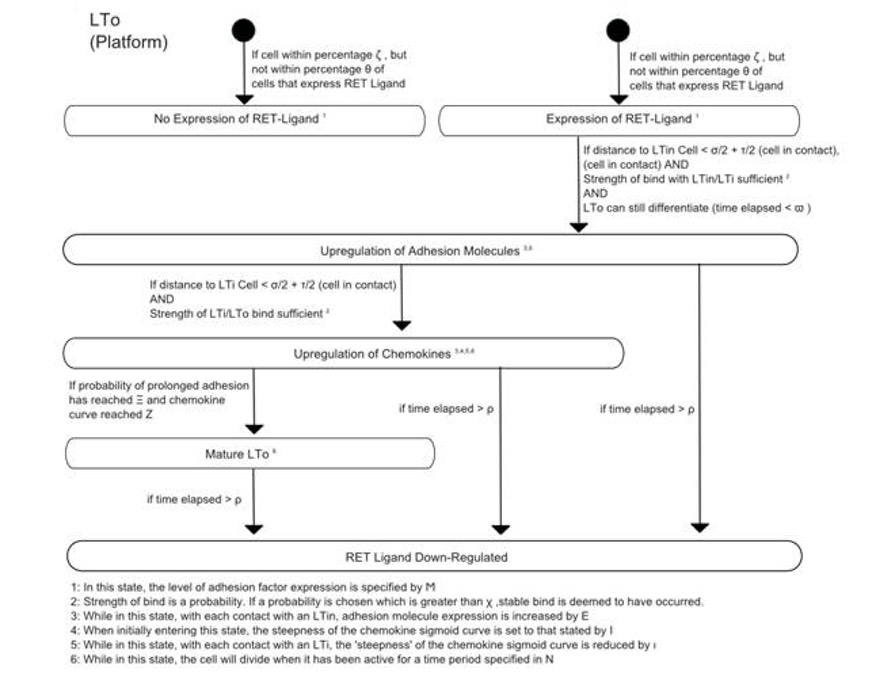
\includegraphics[width=\textwidth]{Appendix/Models/Platform/LTo}
\caption{LTo}
\end{subfigure}

\caption{Platform Model State Diagrams \cite{kieran_thesis, kieran_methodology}}
\label{fig:platform_state_diagrams}
\end{figure}

\begin{figure}[htp]

\begin{adjustbox}{center}
\begin{tabular}{|c p{3.5cm}|c|r|} 
\hline
& \textbf{Parameter} & \textbf{Simulation Variable} & \textbf{Value} \\ 
\hline
$\varsigma$ & \gls{LTin} Cell Input Rate & \textit{Calculated} & 79 cells / 100 steps \\
\hline
\textPsi & \gls{LTi} Input Rate & \textit{Calculated} & 97 cells / 100 steps \\
\hline
\texttau & \gls{LTin} / \gls{LTi} Cell Size & LTI\_CELL\_SIZE & 6 px \\
\hline 
\textsigma & \gls{LTo} Cell Size & LTO\_CELL\_SIZE & 2 px \\
\hline 
\textPi & Simulation Run Cell Speed Lower Bound & \textit{N/A} & 0 \\ 
\hline
\textTheta & Simulation Run Cell Speed Upper Bound & MAX\_CELL\_SPEED & 10 \\ 
\hline
\hline
\textMu & Initial Expression Adhesion Factors & INITIAL\_ADHESION & 0 \\
\hline
\textXi & Linear Equation Slope & ADHESION\_SLOPE & Calibrated to 1 \\
\hline
\textEpsilon & Increase in Adhesion with each stable contact & ADHESION\_INCREMENT & Calibrated to 0.05 \\
\hline
\textnu & Adhesion Level Threshold & MAX\_ADHESION\_PROBABILITY & Calibrated to 0.65 \\
\hline
\hline
\textphi & Chemokine Threshold & CHEMO\_THRESHOLD & Calibrated to 0.3 \\
\hline
\textBeta & Sigmoid Curve Adjustment & CHEMO\_CURVE\_ADJUST & 3 \\
\hline
\textIota & Initial Curve Value & CHEMO\_UPPER\_ADJUST & Calibrated to 0.2 \\
\hline
\textZeta & Lower Curve Value & CHEMO\_LOWER\_ADJUST & Calibrated to 0.04 \\
\hline
\textiota & Increase in expression with stable contact & INCREASE\_CHEMO\_EXPRESSION & Calibrated to 0.005 \\
\hline
\hline
\textKappa & Circumference (Environment growth not implemented) & CIRCUMFERENCE & 254 \\
\hline
\textRho & Length (Environment growth not implemented) & LENGTH & 7303 \\
\hline
\end{tabular}
\end{adjustbox}

\caption{Platform Model Simulation Parameters \cite{kieran_thesis, kieran_methodology}}
\label{table:simulation_params}
\end{figure}
 
\end{document}